\chapter{Metodolog\'ia}

El capítulo anterior hace referencia a las metodologías recientes que son
utilizados para la autonomía de un robot móvil y para la generación de
un mapa bidimensional, dentro de un ambiente aún por conocer. En el presente
trabajo de tesis se ha desarrollado un sistema de movimiento 
autónomo, del robot móvil, basado en campos potenciales, leyes de control 
polar y posiciones aleatorias dentro de un espacio de configuración. Este sistema
permite lograr que el robot pueda explorar un ambiente desconocido de manera
autónoma. Asimismo, también se ha desarrollado un sistema mecánico accionado 
por un motor paso a paso, el cual permite que el robot mientras se va desplazando
dentro de un entorno este pueda tomar mediciones en los tres ejes del plano
cartesiano y así obtener una representación gráfica del lugar en tres 
dimensiones. Estos sitemas pueden ser implementados desde una computadora en 
tiempo real (\textit{online}) o también puede ser implementado por medio de 
un microcontroladore (\textit{onboard}). En este capítulo se explicará, con 
detalles, los métodos que fueron implementados para realizar el presente trabajo.

%En el cap\'itulo anterior se explic\'o sobre las metodolog\'ias recientes que se 
%utilizan para que un robot pueda ser aut\'onomo y genere un mapa 
%del entorno donde se encuentre. En este trabajo de tesis se propone 
%el movimiento aut\'onomo basado en campos potenciales y en leyes de control 
%polar para el movimiento de un robot m\'ovil, de modo que sea capaz de alcanzar 
%un objetivo que vuelva a planificar continuamente su camino sin colisiones. El 
%algoritmo desarrollado puede ser implementado desde una computadora en tiempo 
%real (\textit{online}) o tambi\'en puede ser implementado por medio de un 
%microcontrolador (\textit{onboard}). En este cap\'itulo se explicar\'a, con detalles, 
%los m\'etodos que fueron implementados en este trabajo.

\section{Ejemplo de Aplicación}
En esta sección se explica los componentes que fueron utilizados para construir
el prototipo funcional. Estos componentes se utilizan para la navegación 
autónoma del robot móvil y para tomar medidas en los tres ejes del plano
cartesiano. Para la navegación se utilizó un robot móvil diferencial terrestre, y 
para tomar medidas del entorno se utilizó un sensor lidar.
%En esta secci\'on se explica cada uno de los componentes que tuvo que 
%ser utilizados para realizar la autonom\'ia y el mapeo de este trabajo de 
%tesis. Para realizar la autonom\'ia se utiliz\'o un robot m\'ovil diferencial 
%terrestre, y as\'i tambi\'en para mapear el entorno por donde el robot se 
%desplaza se utiliz\'o un sensor lidar.

%\subsection{Descripci\'on del Robot M\'ovil}
% \begin{figure}%[h]
% \centering \footnotesize
% {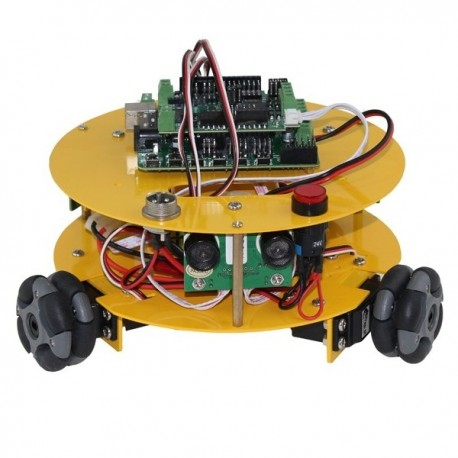
\includegraphics[width=0.40\linewidth]{images/omnidirecional.jpg}}
% \captionsetup{font=footnotesize}
% \caption{Robot m\'ovil hol\'onomico omnidireccional}
% \label{fig:omnidirectional}
% \end{figure}
% \begin{figure}%[h]
% \centering \footnotesize
% {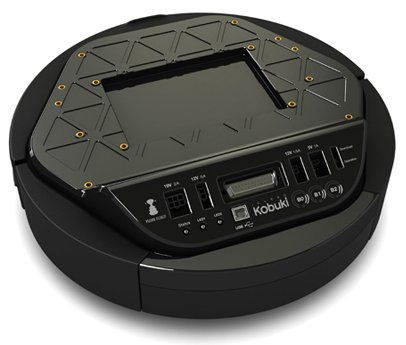
\includegraphics[width=0.40\linewidth]{images/kobuki.jpg}}
% \captionsetup{font=footnotesize}
% \caption{Robot m\'ovil no-hol\'onomico utilizado para implementar el 
% algoritmo de autonom\'ia}
% \label{fig:kobuki}
% \end{figure}
% Una forma de clasificar a los robots m\'oviles es a trav\'es de la locomoci\'on 
% de sus ruedas, esto se divide en dos: (1) robot holon\'omico y (2) robot 
% no-holon\'omico. El robot holon\'omico no tiene ninguna restricci\'on, con 
% respecto a la velocidad, en la posici\'on y la orientaci\'on. El robot se puede 
% mover instant\'aneamente en cualquier direcci\'on del espacio, sin necesidad de 
% rotar previamente. La mayor\'ia de estos robots m\'oviles son omnidireccionales, 
% como se puede ver en la figura \ref{fig:omnidirectional}. En cambio un robot 
% no-holonomico tiene una restricci\'on en su velocidad, no existe un trayectoria 
% que dependa solamente de la posici\'on y orientaci\'on. Por ende, este robot no 
% se puede mover instant\'aneamente en cada direcci\'on del espacio.

%Para este trabajo se hizo uso del robot m\'ovil no-holon\'omico, Kobuki (figura \ref{fig:kobuki})
%el cual esta configurado para poder trabajar con ROS (\textit{Robot Operating System}) 
%con una velocidad de translaci\'on de 70 $cm/s$, una velocidad de rotaci\'on de 180 
%$grados/s$, una posibilidad de carga de hasta 5 $kg$, un tiempo de operaci\'on de 3 
%horas \cite{aboutKobuki}. 

\subsection{Cinem\'atica de Robot M\'ovil Diferencial}
\begin{figure}%[h]
\centering \footnotesize
{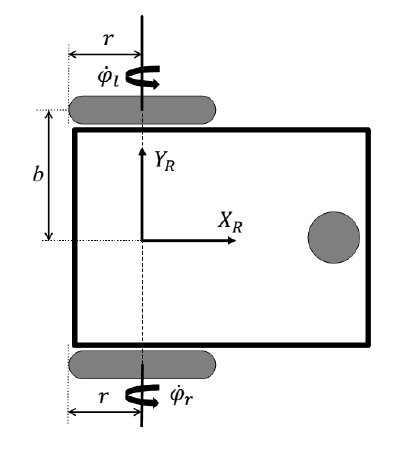
\includegraphics[width=0.40\linewidth]{images/kinematic_model.png}}
\captionsetup{font=footnotesize}
\caption{Representaci\'on gr\'afica de un robot m\'ovil diferencial. Donde 
$b$ es la distancia de su centro de masa hacia sus ruedas, el radio de cada 
rueda es representado por $r$. Finalmente $\dot{\varphi_{l}}$ y 
$\dot{\varphi_{r}}$ son las velocidades de la rueda derecha y rueda izquierda 
correspondientemente.}
\label{fig:RMkinematic}
\end{figure}
Para realizar el modelo cinemático del robot diferencial se debe tener 
en cuenta algunas consideraciones sobre el comportamiento de este. Se asume 
que el robot se desplaza en una superficie plana idealmente sin rozamiento, 
también se toman los ejes de las ruedas como perpendiculares al suelo
por donde se desplaza y que solo existe un punto de contacto entre 
la rueda y el suelo.

%El robot se considera como un cuerpo r\'igido sin partes flexibles, pero se 
%deben tener en cuenta las restricciones no-holon\'omicas. Es decir, el robot 
%puede desplazarse hacia atr\'as o hacia adelante, pero no puede trasladarse 
%hacia los lados. Para poder realizar estos movimientos, se debe realizar un 
%movimiento en partes.

El modelo cinemático del robot necesita conocer las dimensiones del robot. Las 
medidas que se necesitan son la distancia entre las ruedas y el radio de las 
mismas. La distancia entre las ruedas es representada como $2b$ y el radio de 
las ruedas como $r$. También se debe considerar que el robot tiene dos ruedas 
convencionales fijas y el sistema de referencia del robot se encuentra entre 
ambas ruedas, como se ve en la Figura \ref{fig:RMkinematic}.

Teniendo en consideración las restricciones de las ruedas convencionales se halla la 
cinemática directa del robot móvil. La cinemática directa consiste en:
\begin{align*}
v &= \frac{r}{2}(\dot{\varphi_{r}} + \dot{\varphi_{l}}), \\
\omega &= \frac{r}{2b}(\dot{\varphi_{r}} + \dot{\varphi_{l}}),
\end{align*}
donde $v$ es la velocidad lineal y $\omega$ es la velocidad angular. Estas 
velocidades del robot móvil se hallan a 
través de las velocidades de cada rueda del robot. Por otro lado la cinemática inversa 
como dice su nombre es todo lo contrario a la cinemática directa. Este consiste en:
\begin{align*}
\dot{\varphi_{r}} &= \frac{1}{r}(v + b\omega), \\
\dot{\varphi_{l}} &= \frac{1}{r}(v - b\omega),
\end{align*}
donde se halla las velocidades de las ruedas a partir de la velocidad lineal y velocidad
angular del robot móvil.
\begin{figure}%[h]
 \centering \footnotesize
 %{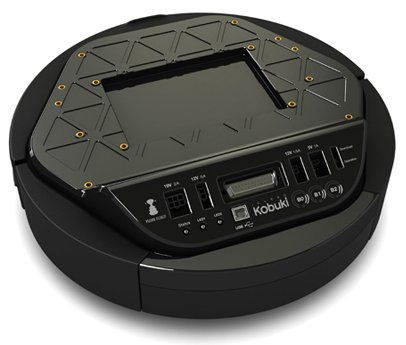
\includegraphics[width=0.35\linewidth]{images/kobuki.jpg}}
 {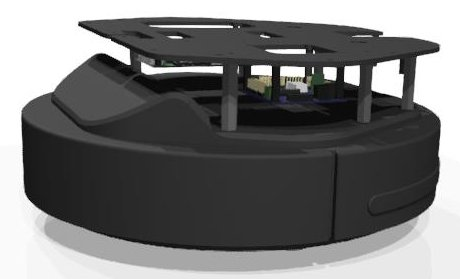
\includegraphics[width=0.35\linewidth]{images/turtlebot.jpg}}
 \captionsetup{font=footnotesize}
 \caption{Representación gráfica del robot móvil diferencial utilizado para la implementación 
 del sistema de navegación aútonoma.}
 \label{fig:kobuki}
 \end{figure}
Para este trabajo se hizo uso del robot móvil no-holonómico, Kobuki (ver Figura 
\ref{fig:kobuki}) el cual trabaja con una velocidad de translación de 70 $cm/s$ y una 
velocidad de rotación de 180 $grados/s$. Tiene una posibilidad de carga de hasta 5 $kg$ y 
un tiempo de operación de 3 horas \cite{aboutKobuki}.
%Para calcular la cinem\'atica del robot m\'ovil se debe usar las restricciones 
%de las ruedas convencionales. Las restricciones de cada rueda fija son:
%\begin{equation*}
%\[-\text{sin}(\alpha + \beta) & \text{cos}(\alpha + \beta) & \text{lcos}(\beta)\] 
%{R}^R_{I} {I}^\dot{\xi} - r\dot{\varphi} &= 0 \\
%\[\text{cos}(\alpha + \beta) & \text{sin}(\alpha + \beta) & \text{lsin}(\beta)\]
%{R}^R_{I} {I}^\dot{\xi} &= 0
%\end{equation}
%donde ${R}^R_{I}$ es la matriz de rotaci\'on que lleva el sistema de coordenadas del 
%robot $(X_{R},Y_{R})$ al sistema inercial $(X_{I},Y_{I})$ y $\dot{\xi}$ 
%es el vector que contiene los valores de las velocidades lineales y angular 
%del robot.


\subsection{Sistema de Percepción Bidimensional}
\begin{figure}%[h]
	\centering \footnotesize
 	{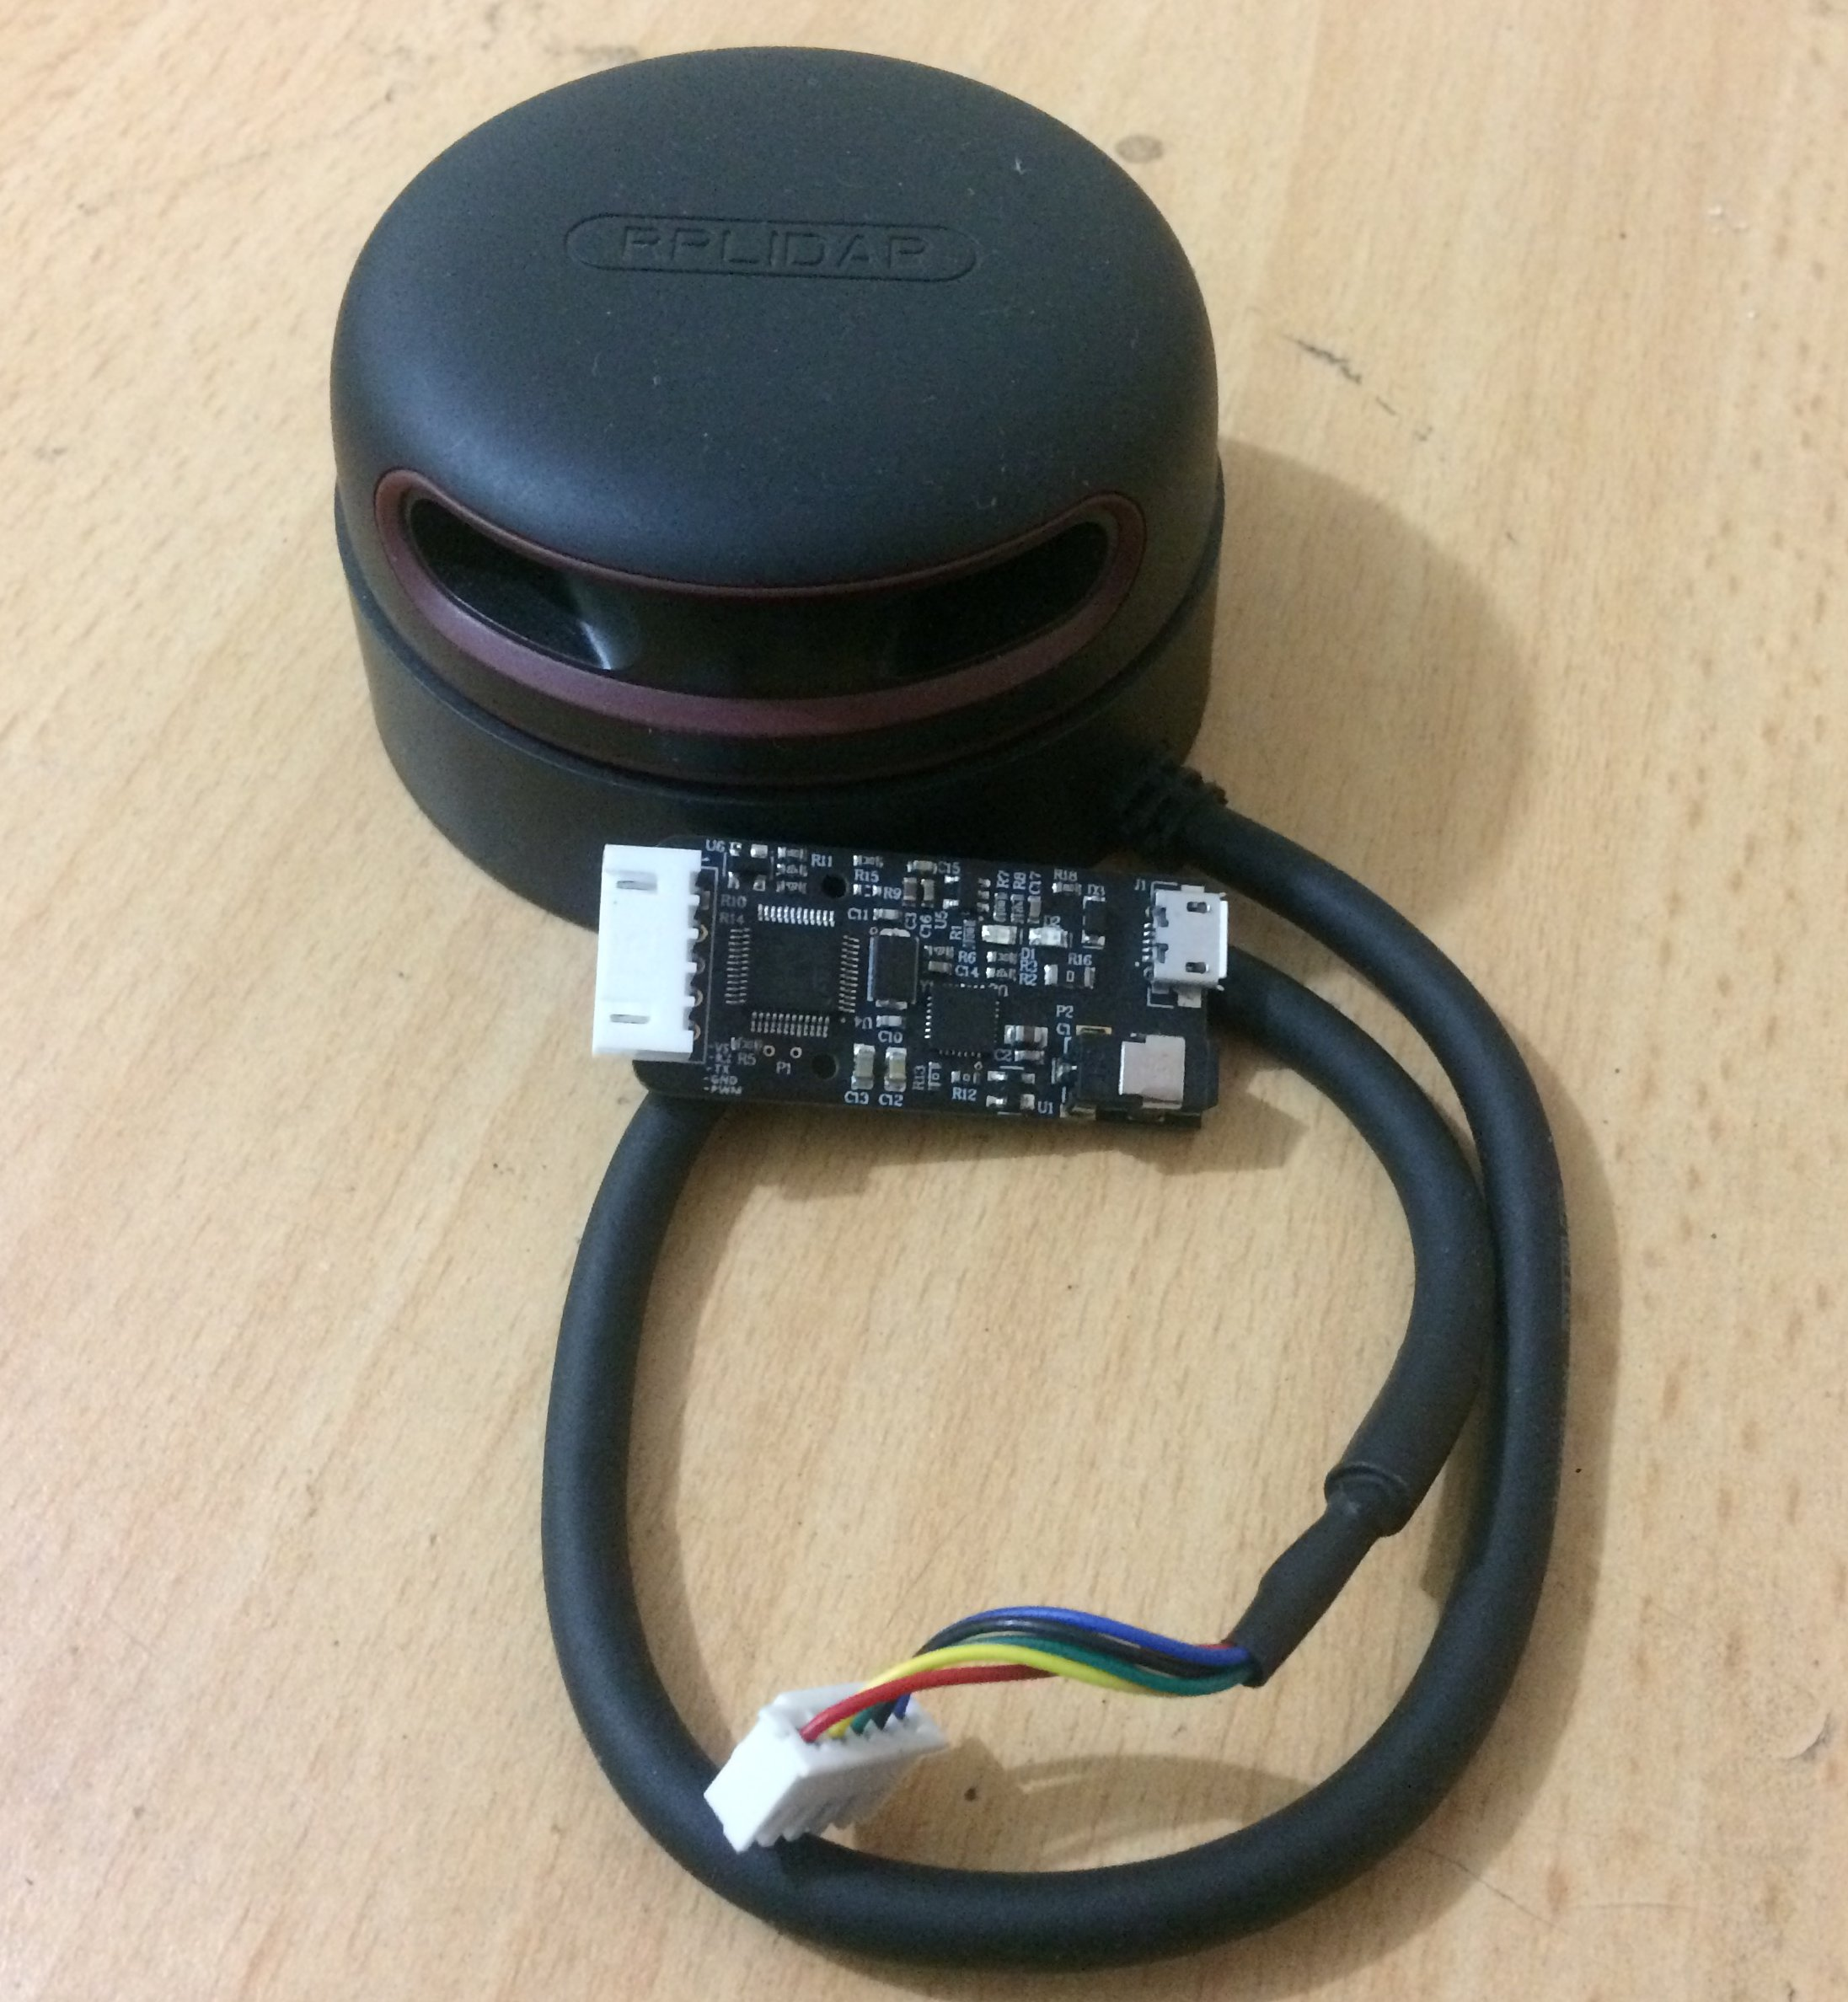
\includegraphics[width=0.60\linewidth]{images/rplidar.JPG}}
 	\captionsetup{font=footnotesize}
 	\caption{Sensor lidar RPLIDAR A2 \cite{sensorLidar}.}
 	\label{f:lidar}
\end{figure}

Para generar el mapa de un entorno, se necesita medir distancias del ambiente y así
generar el mapa. En este trabajo se utiliza un sensor lidar RPLidar A2 el cual se basa en 
el principio de rango de triangulación láser \cite{amann2001laser} y ha sido desarrollado 
por la empresa \textit{SLAMTEC}.

El sensor lidar es un sensor que no necesita tener una luz externa para poder obtener las
medidas de las distancias. Este sensor tiene un láser infrarrojo de baja potencia el cual
es controlado por medio de un pulso modulado. Este sensor puede girar en 360\grad ~y tiene
un rango de alcance máximo de 6 metros. Trabaja a una frecuencia de 10Hz teniendo una tasa 
de medición de 4000 muestras por segundo. La transmisión de datos de este sensor es por 
medio de un protocolo UART. El sensor es mostrado en la Figura \ref{f:lidar}.


%Es un sensor l\'aser que se basa en el  principio de rango de triangulaci\'on 
%láser \cite{amann2001laser} y adopta el hardware de adquisici\'on y 
%procesamiento de visi\'on de alta velocidad desarrollado por \textit{SLAMTEC}. El 
%sensor utiliza un l\'aser infrarrojo de baja potencia como su fuente de luz y lo 
%maneja utilizando un pulso modulado. Este sensor gira a 360 \grad ~y llega a 
%una distancia m\'axima de 8 metros. Trabaja a una frecuencia de 10 Hz y 
%tiene una tasa de medici\'on de 4000 muestras por segundo. El hardware del 
%RPLIDAR A2 se puede ver en la figura \ref{f:lidar}, el cual tiene un 
%convertidor de protocolo UART a mini USB.


\begin{table}[htbp]
\begin{center}
\begin{tabular}{|l|c|c|c|c|}
	\hline
	Item & Unidad & M\'inimo & T\'ipico & M\'aximo\\
	\hline \hline
	Rango de distancia & m & 0.15 & - & 6 \\ \hline
	Rango angular & grados & - & 0 - 360 & - \\ \hline
	Resoluci\'on de la distancia & mm & - & menor a 0.5 & - \\ \hline
	Duraci\'on de muestra & ms & - & 0.25 & - \\ \hline
	Resoluci\'on angular & grados & 0.45 & 0.9 & 1.35 \\ \hline
	Fecuencia de muestreo & Hz & 2000 & 4000 & 4100 \\ \hline
	Frecuencia de escaneo & Hz & 5 & 10 & 15 \\ \hline
\end{tabular}
	\caption{Pruebas de Medici\'on del sensor RPLidar A2.}
	\label{tbl:medicion}
\end{center}
\end{table}

La Tabla \ref{tbl:medicion} muestra el rendimiento de medici\'on del 
sensor lidar \cite{Slamtec} considerando varias pruebas por cada variable. Las variables más 
importantes de esta Tabla son: (i) Rango de distancia, el sensor toma mediciones en el
rango mostrado, cuando la distancia es menor a 0.15 $mts$ no considera la medición, lo 
mismo sucede cuando la medición es mayor a 8 $mts$. (ii) Resolución de la distancia, el 
sensor tiene un error menor a 0.5 $mm$ en sus mediciones, esto permite construir un mapa 
con las dimensiones reales del entorno.(iii) Resolución angular, este sensor tiene una 
resolución de 1\grad~ esto quiere decir que por cada grado que gira el lidar esta realizando 
una medición, por lo tanto el sensor mide 360 veces por cada rotación.

\begin{figure}
	\centering \footnotesize
	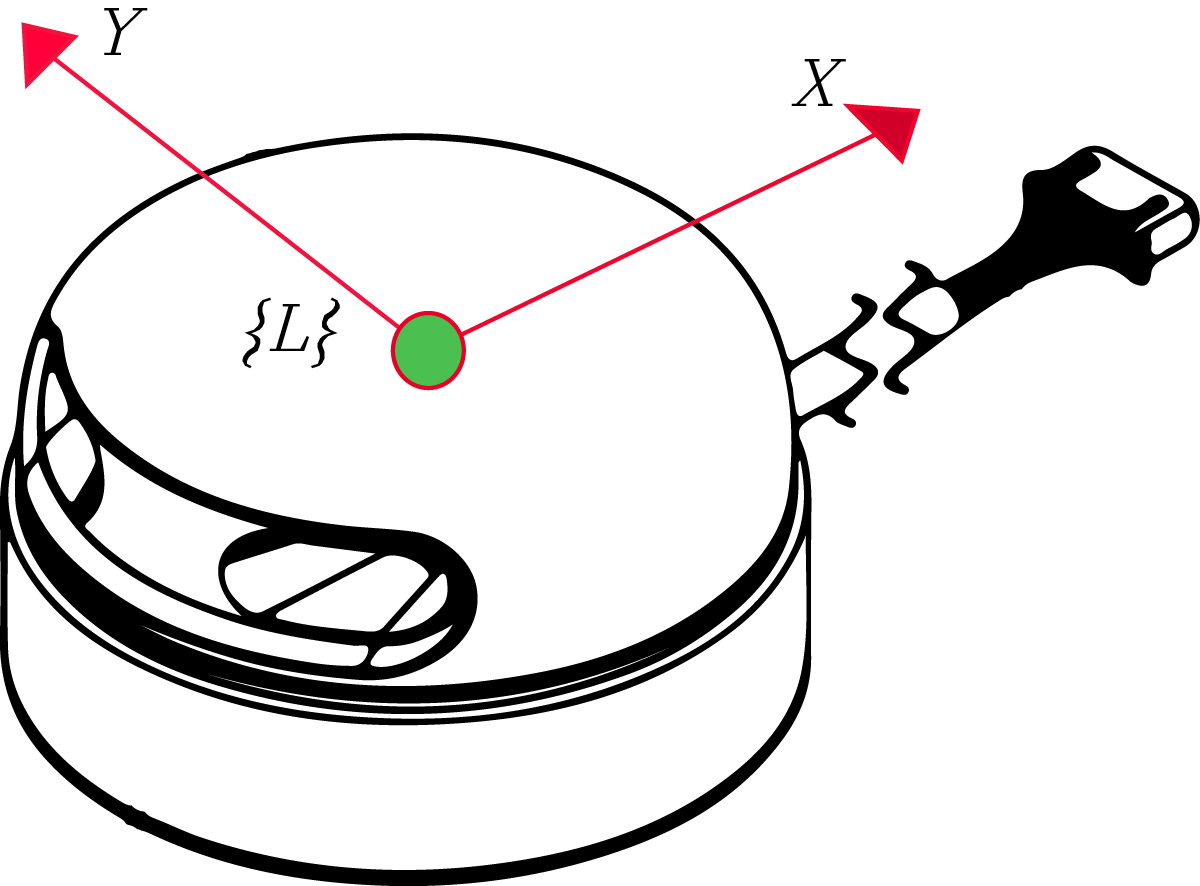
\includegraphics[width=0.40\linewidth]{images/frame_laser.png}
	\captionsetup{font=footnotesize}
	\caption{En esta figura el punto verde representa el sistema de referencia 
	del sensor RPLidar A2, donde el eje $\mayusx$ va en el mismo sentido del cable 
	de datos del sensor lidar.}
	%\caption{Sistema de referencia del sensor RPLidar A2.}
	\label{fig:FrameLidar}
\end{figure}

Para el envío de los datos a la computadora o al microcontrolador, el sensor trabaja con un 
protocolo de comunicación UART. Este protocolo se especifíca en la Tabla \ref{tbl:comunicacion} y 
por medio del protocolo se obtiene los datos de las distancias que mide el sensor. Para construir 
el mapa en dos dimensiones se tiene que tomar en consideración el sistema de referencia del sensor 
lidar. En la Figura \ref{fig:FrameLidar} se puede ver que el cable de comunicación 
indica la dirección del eje $\mayusx$ y al lado derecho se encuentra posicionado el eje 
$\mayusy$. Teniendo en consideración el sistema de referencia del sensor se puede obtener 
las distancias del entorno que se esta midiendo y a partir de una conversión de coordenadas 
polares a coordenadas cartesianas se estima las posiciones de los objetos que se encuentran dentro 
del entorno de trabajo.

\begin{table}[htbp]
\begin{center}
\begin{tabular}{|c|c|c|c|c|c|}
	\hline
	Color & Nombre de la señal & Tipo & Mínimo & Típico & Máximo \\ 
	\hline \hline
	Rojo & VCC & Potencia & 4.9V & 5V & 5.5V \\ \hline
	Amarillo & Tx & Salida & 0V & 3.3V & 3.5V \\ \hline
	Verde & Rx & Entrada & 0V & 3.3V & 3.5V \\ \hline
	Negro & GND & Potencia & 0V & 0V & 0V \\ \hline
	Azul & MOTOCTL & Entrada & 0V & 3.3V & 5V \\ \hline
\end{tabular}
	\caption{Interfaz de comunicación del sensor RPLidar A2.}
	\label{tbl:comunicacion}
\end{center}
\end{table}


\subsection{Sistema de Percepción Tridimensional}
\label{sec:SistP3D}
\begin{figure}[ht!]
     \begin{center}
        \subfigure[]{\label{fig:lidar3Da}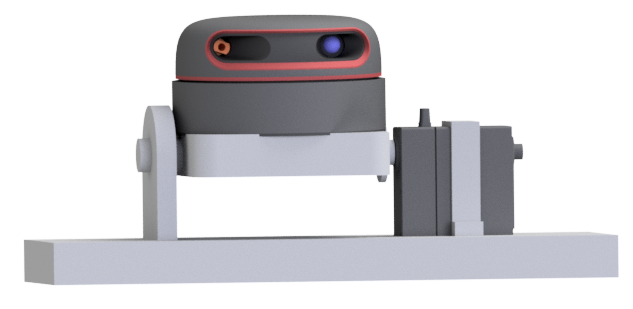
\includegraphics[width=.45\textwidth]{images/lidar_3d.png}}
        \subfigure[]{\label{fig:lidar3Db}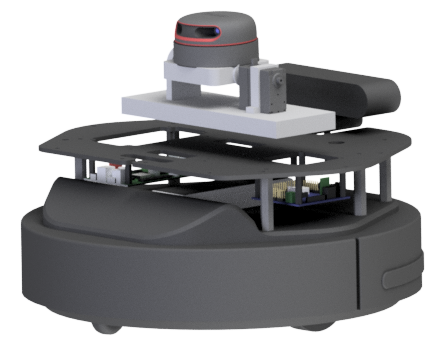
\includegraphics[width=.45\textwidth]{images/lidar_wKbki.png}}
    \end{center}
  \captionsetup{font=footnotesize}
    \caption{\label{f:lidar3D}Diseño del sistema mecánico, desarrollado en un programa CAD. En (a) se 
    muestra el diseño en CAD del sistema mecánico y en (b) se muestra la forma en que va ser colocado 
    el sistema mecánico en el robot móvil kobuki.}
\end{figure}
%\begin{figure}%[ht!]
%  	\centering \footnotesize
  %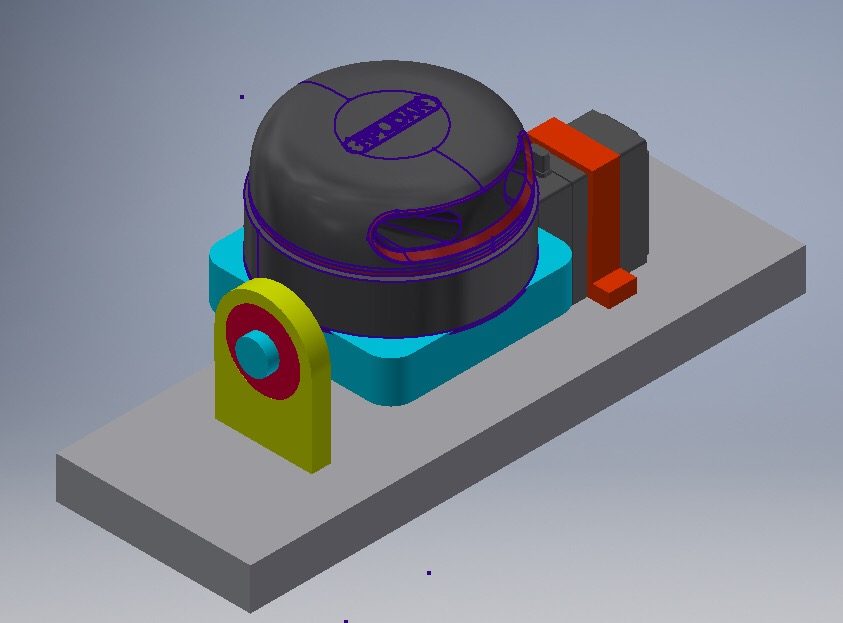
\includegraphics[width=0.40\textwidth]{images/lidar_3D.jpeg}
  %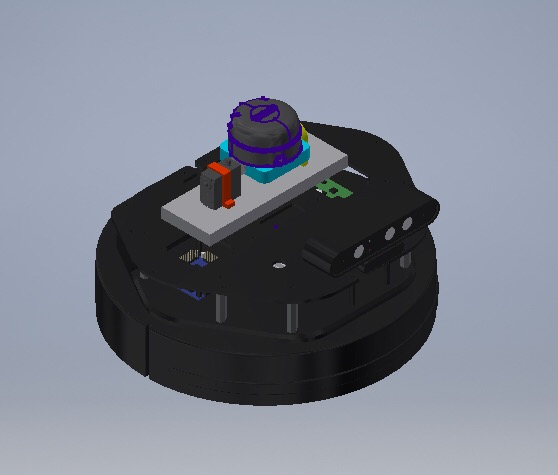
\includegraphics[width=0.35\textwidth]{images/kbki_lidar3D.jpeg}
%  	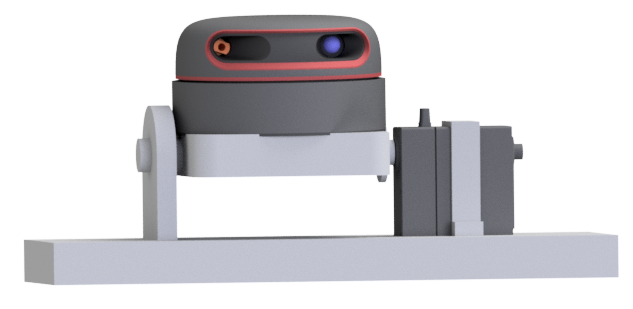
\includegraphics[width=0.40\textwidth]{images/lidar_3d.png}
%  	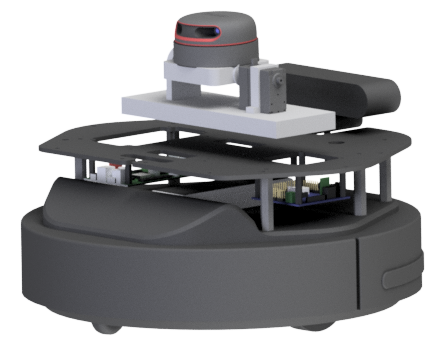
\includegraphics[width=0.40\textwidth]{images/lidar_wKbki.png}
%  	\\ $\qquad\qquad$ a. Sistema mecánico  $\qquad\qquad\qquad$  b. Sistema mecánico sobre el Kobuki
%  	\captionsetup{font=footnotesize}
%  	\caption{Sistema mec\'anico para el mapeo en tres dimensiones.}
%  	\label{f:lidar3D}
%\end{figure}

El sensor lidar permite construir mapas en dos dimensiones ya que este va midiendo 
distancias mientras va rotando en 360\grad ~, pero para el alcance de este proyecto de 
tesis se necesita que el robot pueda mapear el entorno en tres dimensiones. Para este
objetivo se realizó un diseño mecánico, como se muestra en la Figura \ref{f:lidar3D}a. Este
diseño permite que el sensor lidar pueda tener un ángulo de medición de $\pm$ 15\grad en el 
eje $Z$. El sistema mecánico consiste en una base donde el sensor lidar se encuentra acoplada, 
y a su vez este esta unido a un servomotor por medio de un eje. El servomotor esta programado para 
que se mueva en un rango de $\pm$ 15\grad~ para que el sensor pueda tomar medidas 
en el eje $Z$. 

\begin{figure}[ht!]
     \begin{center}
        \subfigure[]{\label{fig:etiquetaB}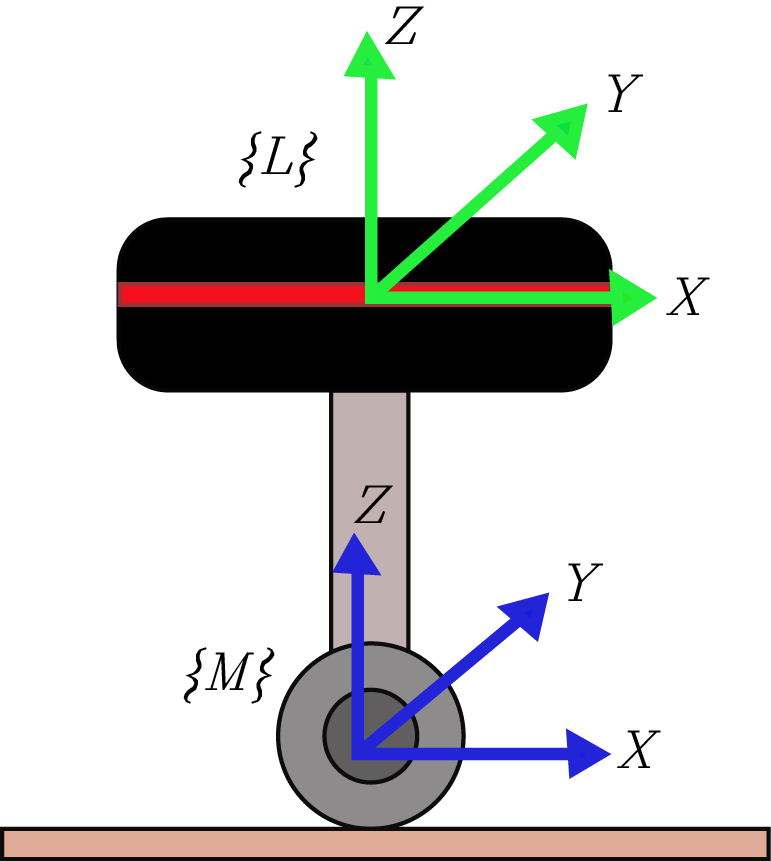
\includegraphics[width=.47\textwidth]{images/lidar_ref.png}}
        \subfigure[]{\label{fig:etiquetaC}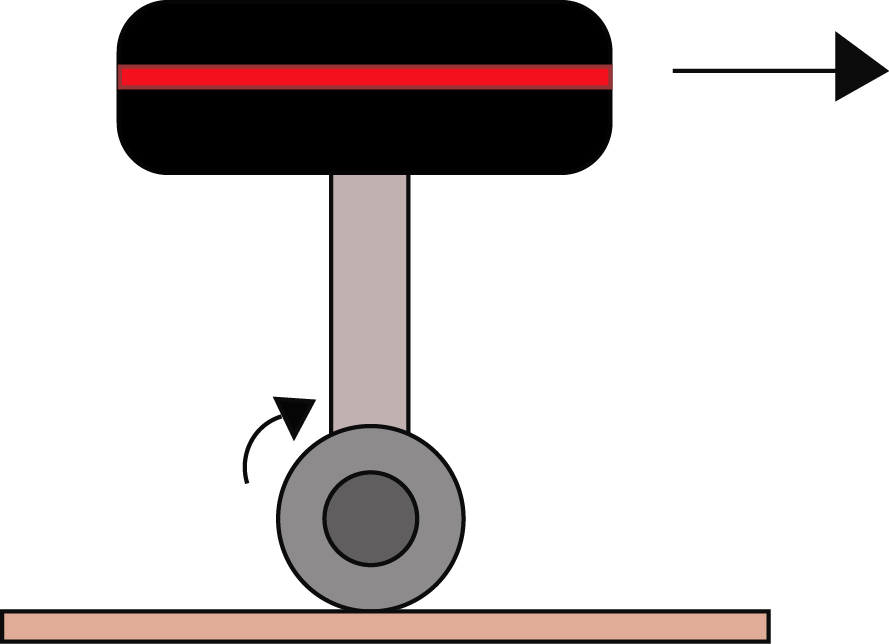
\includegraphics[width=.50\textwidth]{images/lidar_giro.png}}
    \end{center}
  \captionsetup{font=footnotesize}
    \caption{\label{f:Rot3D}Representación gráfica de los movimientos de rotación y traslación 
    del sistema mecánico, en (a) se muestra los sistemas de referencia del motor y del sensor 
    lidar. En (b) se muestra el movimiento de rotación originado por el motor y el movimiento 
    de traslación del sensor lidar, para tomar las mediciones en los tres ejes del plano cartesiano.}
\end{figure}

%\begin{figure}%[ht!]
%	\centering \footnotesize
%	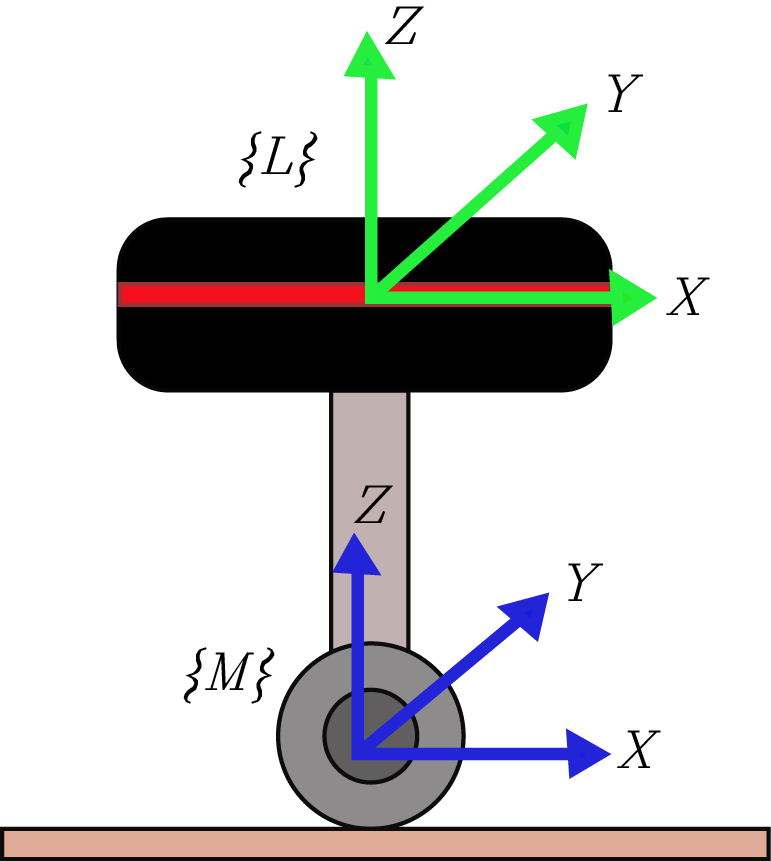
\includegraphics[width=0.40\textwidth]{images/lidar_ref.png}~~~~~~~~~~~~
%	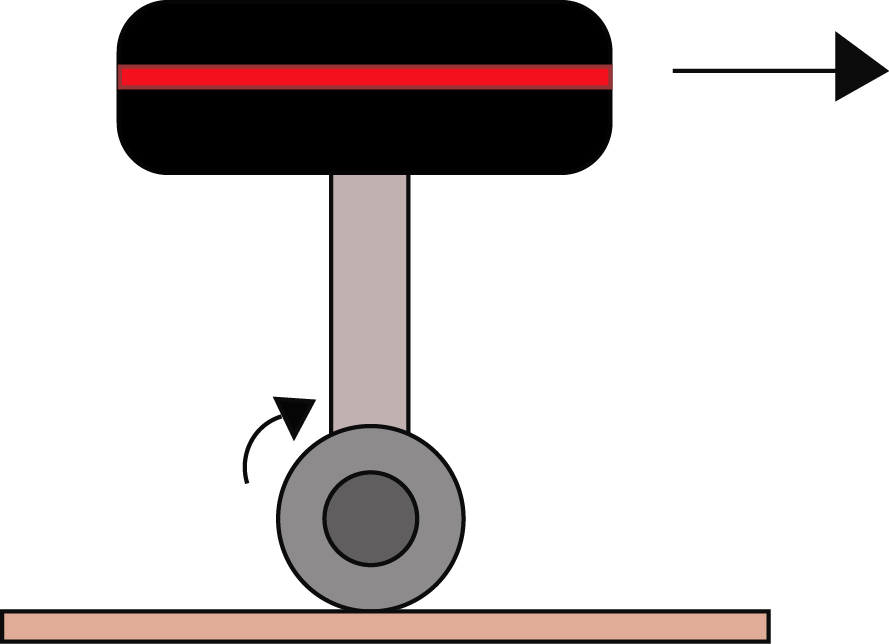
\includegraphics[width=0.40\textwidth]{images/lidar_giro.png}
%	\\ a. Sistemas de referencia ~~$\qquad\qquad\qquad$~~ b. Rotación y traslación 
%	\captionsetup{font=footnotesize}
%  	\caption{Representación de la rotación y traslación del sistema mecánico}
%  	\label{f:Rot3D}
%\end{figure}

El sistema mecánico esta compuesto por dos sistemas de referencia, el primero es el sistema 
del servomotor y el segundo el sistema del sensor lidar (ver Figura \ref{f:Rot3D}a). Este sistema
genera dos tipos de movimiento uno de rotación y el otro de traslación los cuales son considerados
en la generación del mapa en tres dimensiones (ver Figura \ref{f:Rot3D}b). Para construir el mapa en 
tres dimensiones se debe considerar las distancias que mide el lidar el ángulo que rota el 
servomotor, para esto primero se debe convertir los puntos del lidar en dos dimensiones 
($x,y$). Las ecuaciones para la conversión son:
\begin{align*}
	x &= rcos(\theta_{L}) \\
	y &= rsen(\theta_{L})
\end{align*}
donde $r$ es la distancia medida por el sensor y $\theta_{L}$ es el ángulo que gira el sensor 
mientras va midiendo.

Para llevar la nube de puntos al sistema de referencia del servomotor se utiliza una matriz 
homogénea que contiene las componentes de rotación y traslación del sistema mecánico. La transformación
homogénea esta representada como:
\begin{align*}
	T_{L}^{M} &= R_{y}(\phi_{M}) T_{z}(d), \\
\end{align*}
%\begin{align}
%	\tilde{p}^{M} = T_{L}^{M} \tilde{p}^{L}
%	\label{eqn:MatrizHomogenea}
%\end{align}
donde $\phi_{M}$ es el ángulo que rota el servomotor y $d$ es la distancia que hay entre el sistema de 
referencia del servomotor y el sistema de referencia del sensor lidar, como se puede ver en la 
figura \ref{f:Rot3D} a. $T_{L}^{M}$ es la matriz de transformación homogénea del sistema mécanico. Esta 
matriz tiene una matriz de rotación ($R_{y}(\phi_{M})$) originado por el servomotor en el eje $Y$ y una
matriz de traslación ($T_{Z}(d)$) en el eje $Z$ originado por eje que une el servomotor con el sensor 
lidar.La posición y orientación de la nube de puntos es representada como:
\begin{align}
	\tilde{p}^{L} = T_{L}^{M} \tilde{p}^{M}
	\label{eqn:MatrizHomogenea}
\end{align}
donde $\tilde{p}^{L}$ es la coordenada homogénea con respecto al sistema de referencia del sensor
lidar, $T_{L}^{M}$ es la matriz homogénea descrita anteriormente y $\tilde{p}^{M}$ es la coordenada 
homogénea con respecto al sistema de referencia del servomotor. La multiplicación de estas matrices
ayuda a poder encontrar los puntos en los ejes ($X,Y,Z$) y formar la nube de puntos en el plano 
cartesiano.

\subsection{Prototipo Final}
\begin{figure}%[ht!]
	\centering \footnotesize
	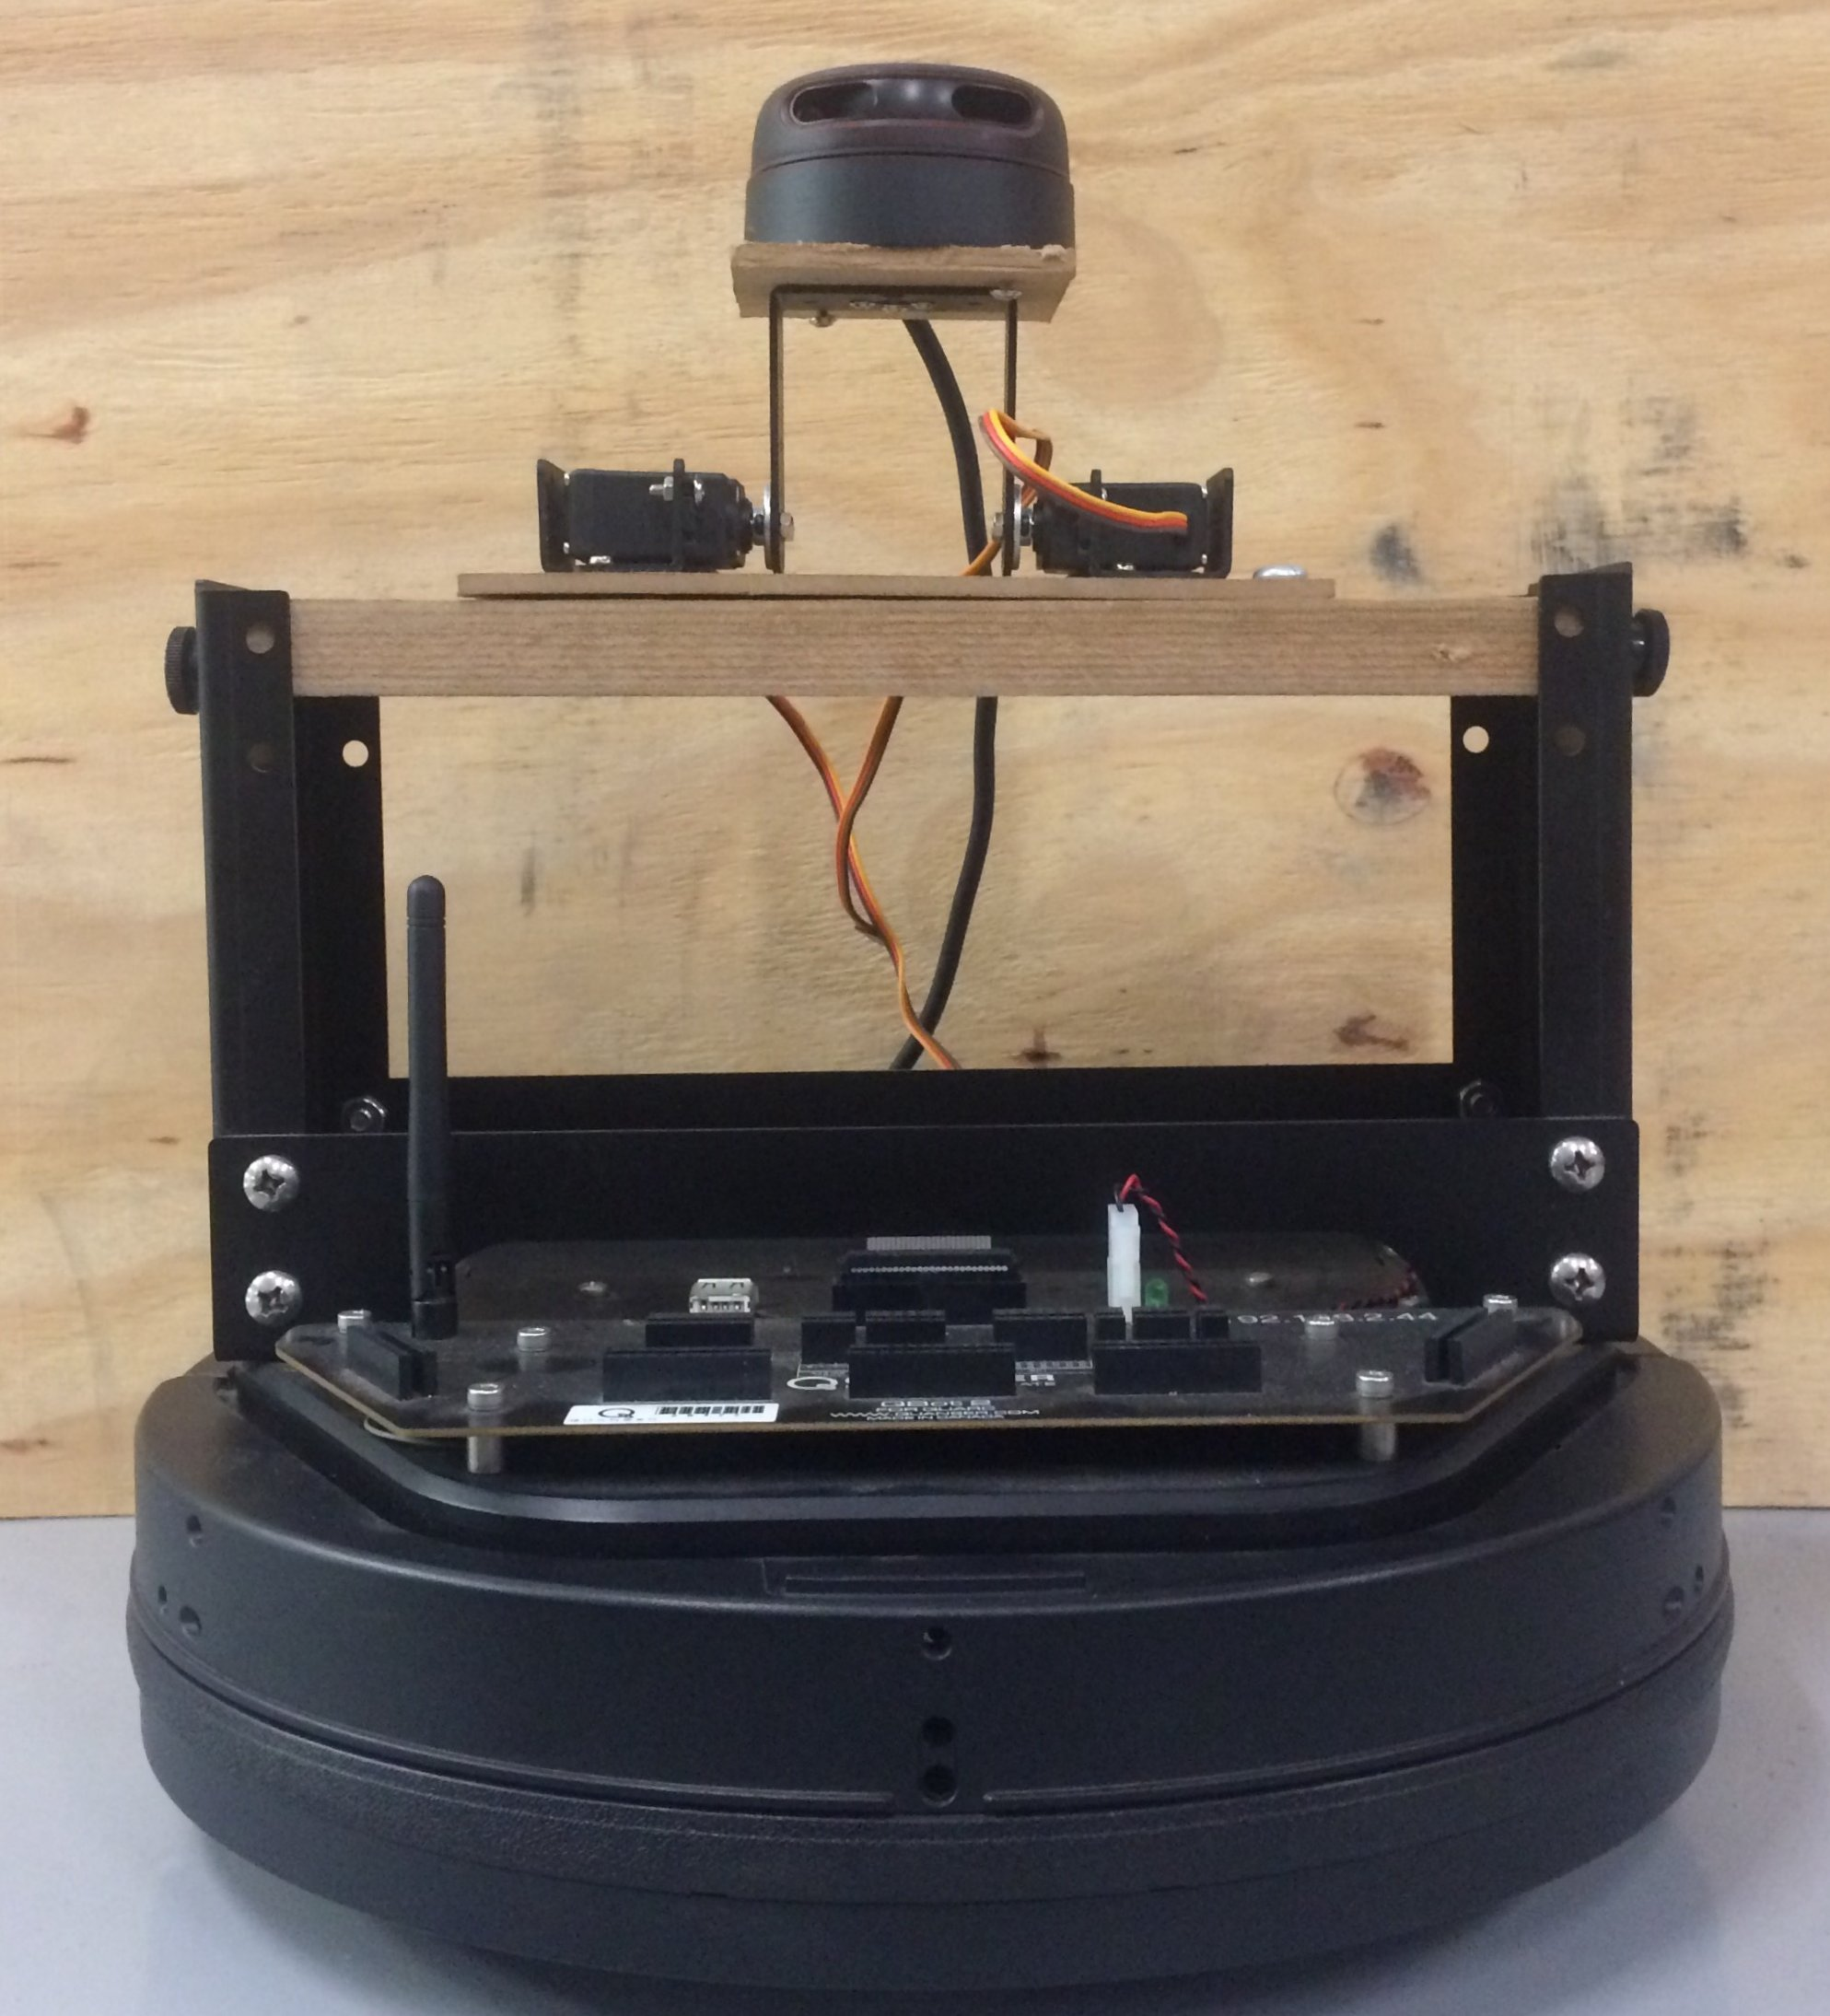
\includegraphics[width=0.40\textwidth]{images/kbkiReal3D.jpg}
	\captionsetup{font=footnotesize}
	\caption{Esta figura muestra el prototipo utilizado donde fue }
	\label{fig:ProtoFinal}
\end{figure}
El prototipo final de este trabajo, permite que el robot pueda generar un mapa en tres dimensiones 
mientras genera su propia trayectoria. La figura \ref{fig:ProtoFinal} muestra el prototipo. Utilizando
un robot diferencial Kobuki conectado al sensor lidar se puede desplazar de forma autónoma
dentro del entorno. El sistema mecánico descrito hace que se genere el mapa en tres dimensiones
y también en dos dimensiones, el cual permitirá que el robot pueda localizarse dentro del ambiente.

%\section{Movimiento del Robot y Mapeo}

%\subsection{Control de Bajo Nivel}

\section{Generaci\'on de Trayectoria basado en Campos Potenciales}
\label{sec:autonomia}

\begin{figure}[ht!]
     \begin{center}
        \subfigure[Fuerzas de atracción]{\label{fig:etiquetaB}\includegraphics[width=.49\textwidth]{images/attr_force.png}}
        \subfigure[Fuerzas de repulsión]{\label{fig:etiquetaC}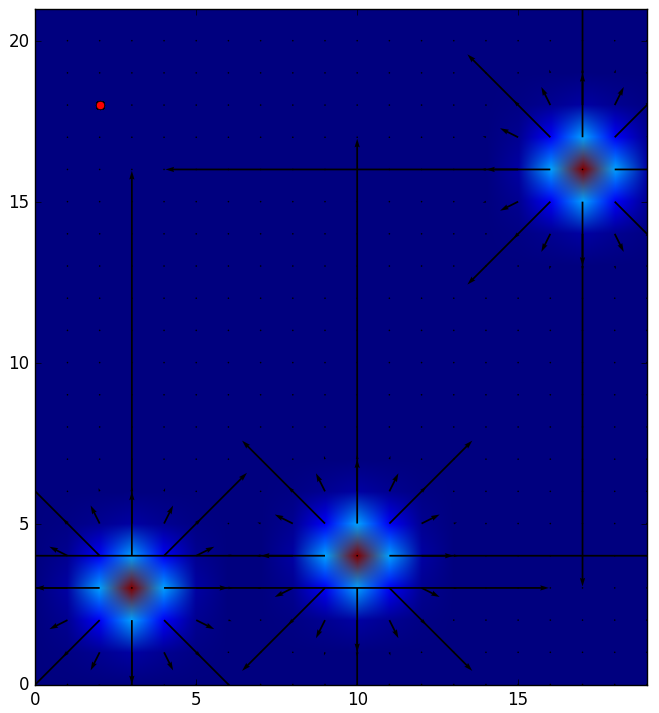
\includegraphics[width=.49\textwidth]{images/rep_force.png}}
        \subfigure[Fuerzas de navegación]{\label{fig:etiquetaC}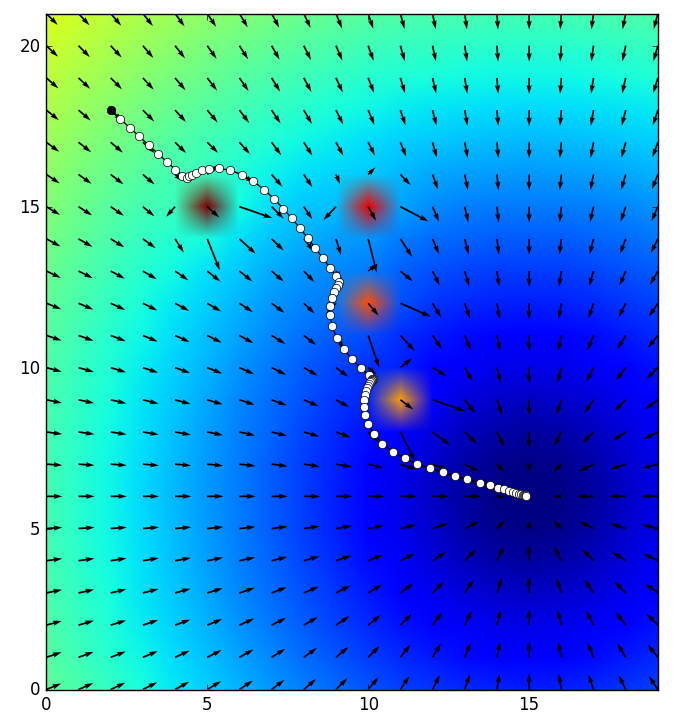
\includegraphics[width=.49\textwidth]{images/nav_force.png}}
    \end{center}
  \captionsetup{font=footnotesize}
    \caption{\label{f:APF}Pruebas para el algoritmo de campo potencial artificial.}
\end{figure}
%\begin{figure}%[ht!]
%  	\centering \footnotesize
  %\subfloat[Attractive Force]{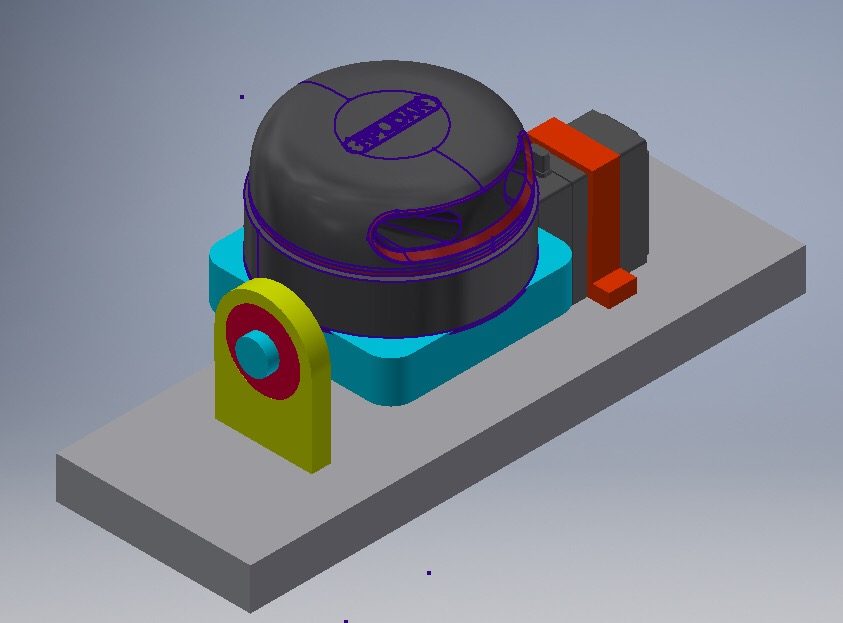
\includegraphics[width=0.16\textwidth]{images/lidar_3D.jpeg}}
  %~\subfloat[Repulsive Force]{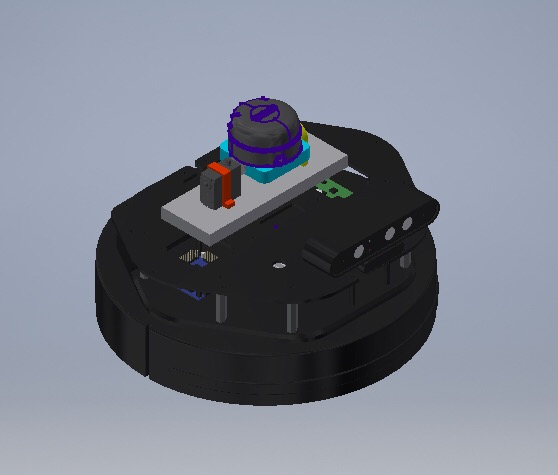
\includegraphics[width=0.16\textwidth]{images/kbki_lidar3D.jpeg}} 
%  	\includegraphics[width=0.40\textwidth]{images/attr_force.png}
%  	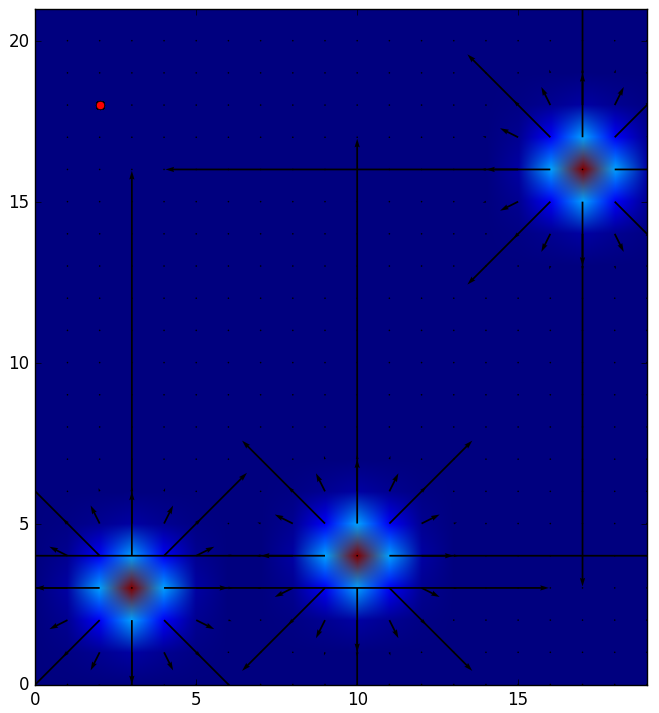
\includegraphics[width=0.40\textwidth]{images/rep_force.png}
%  	\\ $\qquad$ a. Fuerzas de atracción  $\qquad\qquad\qquad$  b. Fuerzas de repulsión
%  	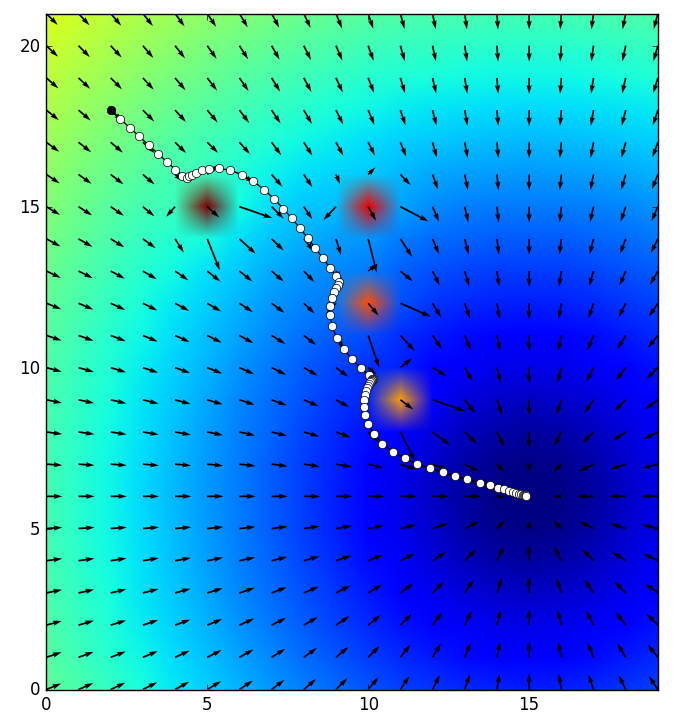
\includegraphics[width=0.45\textwidth]{images/nav_force.png}
%  	\\ $\qquad$ c. Fuerzas de navegación
  %\subfloat[Navigation Force]{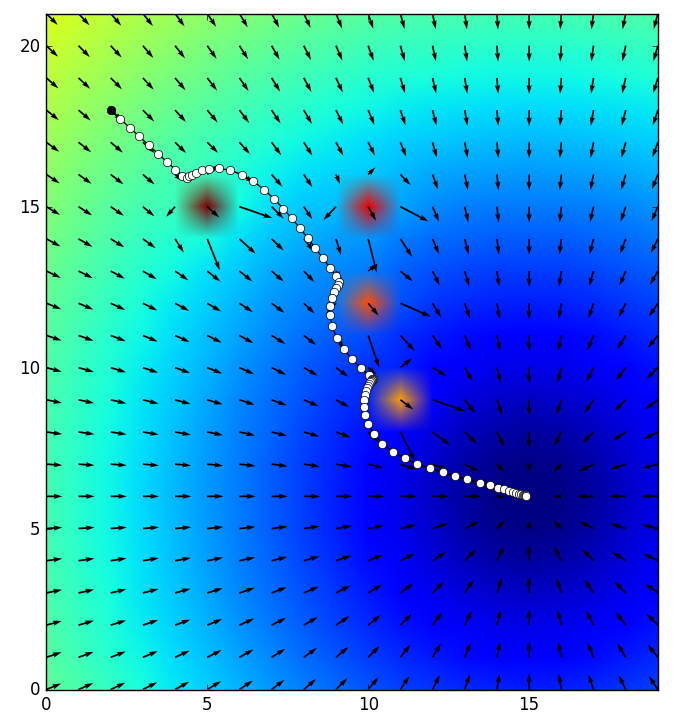
\includegraphics[width=0.16\textwidth]{images/nav_force.png}}
  % \subfloat[Attractive Force]{\includegraphics[width = 150mm]{attr_force.png}}
%  	\captionsetup{font=footnotesize}
%  	\caption{Pruebas para el algoritmo de campo potencial artificial.}
  %\label{f:lidar3D}
%  	\label{f:APF}
%\end{figure}
Para hacer que el robot se mueva a su objetivo final sin toparse con obstáculos, se 
toma el siguiente enfoque. Primero, un objetivo final deseado $q_{g} =(x_{g}, y_{g}, 
\theta_{g})$ que describe la posición y la orientación se específica en términos del 
marco inercial. Entonces, los datos locales actuales del entorno se obtienen por medio 
de un sensor como un lidar, que fue usado en los experimentos, pero se puede usar cualquier 
otro sensor de profundidad. Estos datos proporcionan las posiciones de los obstáculos que 
se encuentran en el campo de visión del robot, y se utilizan como posiciones de obstáculos 
que definen el campo de repulsión.

Usando el campo potencial definido por la posición deseada y los datos detectados, se toma un paso 
en la posición actual. Este paso da un pequeño incremento en la dirección y define la 
posición deseada que debe seguir el controlador polar. A medida que el robot se mueve, esta 
posición deseada también cambia según el campo potencial, guiando el movimiento hacia la meta 
y evitando los obstáculos. A medida que el robot se mueve, continúa escaneando y actualizando 
su mapa de obstáculos y, por lo tanto, actualizando todo el campo potencial compuesto por las 
partes atractivas y repulsivas.

Las fuerzas proporcionadas por el campo de potencial artificial se descomponen en 
magnitud y dirección que conducen continuamente al robot. Para mostrar cómo funciona el 
enfoque, se realiza una prueba en la computadora, que utiliza obstáculos 
colocados artificialmente y una posición deseada. La figura \ref{f:APF} (a) muestra el campo 
de atracción y las fuerzas que guían hacia la posición deseada. El robot simulado se 
encuentra inicialmente en la esquina superior izquierda $q_{0} = (2,18)$ y se mueve hacia 
la meta $q_{goal} = (10,4)$ guiado por el campo. Los puntos blancos muestran la ruta que debe 
seguir el robot y que luego guiará al controlador. Un campo repulsivo puro se muestra en 
\ref{f:APF} (b), donde se agregaron tres obstáculos en diferentes posiciones del espacio de 
trabajo. Cada obstáculo se proyecta como un círculo rojo debido a su gran magnitud dentro de 
su campo potencial, donde las fuerzas apuntan hacia afuera en cada obstáculo. La fuerza de 
navegación total compuesta por la superposición de las fuerzas de atracción y repulsión se 
muestra en la figura \ref{f:APF} (c).

\section{SLAM basado en Filtros de Part\'iculas}

Los filtros de partículas es un método que fue introducido en años recientes como un medio 
eficaz para resolver el problema de la localización y mapeo simultáneo 
\cite{nummiaro2003adaptive}. Para este trabajo de tesis se utilizo un paquete de código 
abierto llamado \textit{gmapping}, este paquete de \textit{ROS} (\textit{Robot Operating System}) 
emplea una técnica llamada \textit{Rao-Blackwellized} basado en filtros de partículas 
\cite{grisetti2007improved}.

El filtro de partículas \textit{Rao-Blackwellized} consiste en que cada partícula 
lleva la información de un mapa del entorno. El cual se enfoca en calcular la 
probabilidad del mapa no solo utilizando la odometría del robot, sino también incluye las 
mediciones que hace un sensor, en este caso un sensor lidar que se encuentra encima del 
robot. Estas informaciones enviadas al algoritmo hace que la incertidumbre sobre la 
posición y orientación del robot disminuya. 

Uno de los principales problemas de la técnica \textit{Rao-Blackwellized} es la cantidad 
de partículas requeridas para construir un mapa preciso. Este efecto es conocido como el 
problema del agotamiento de partículas. Por tal motivo el paquete \textit{gmapping} propone 
dos pasos para solucionar este problema. El primero consiste en calcular la probabilidad 
alrededor de la posición y orientación del robot dependiendo de la cantidad de partículas 
obtenidas mediante los datos del sensor láser. Como fue mencionado anteriormente al tener 
la información del sensor láser y la odometría se puede obtener un mapa corregido y más 
preciso, además el error de estimación de la posición del robot disminuye con el tiempo y 
se requiere menos partículas para representar las futuras posiciones del robot dentro del 
entorno. El segundo paso consiste en un remuestreo adaptativo el cual permite un remuestreo 
cada vez que es necesario, manteniendo una cantidad razonable de partículas. Con este paso 
el paquete \textit{gmapping} reduce el problema del agotamiento de partículas.


\section{Implementaci\'on del sistema}

La metodología propuesta fue probada en un robot móvil Kobuki real, que es un robot de 
accionamiento diferencial, y un \textit{RPlidar} conectado a él. La interfaz entre ambos elementos 
se realizó utilizando un \textit{Raspberry Pi3}, con \textit{ROS} previamente instalado.
El algoritmo fue implementado en el lenguaje \textit{Python}, usando la librería 
\textit{rospy}. Usando este sistema operativo, también es posible transmitir en línea los 
datos adquiridos a una computadora externa. 

\subsection{Sistema Operativo del Robot (ROS)}
ROS es un framework que se usa ampliamente en rob\'otica. Lo que busca este sistema 
operativo de código abierto es hacer una parte del software que pueda funcionar en 
otros robots con solo pequeños cambios en el código. Lo que se obtiene con esta idea 
es la capacidad de crear funcionalidades que se puedan compartir y usar en otros robots, por 
lo que ya no se necesita volver a reinventar la rueda.

Muchas instituciones de investigaci\'on han comenzado a desarrollarse en 
ROS, agregando hardware y compartiendo su c\'odigo. Los sensores y actuadores 
utilizados en la rob\'otica tambi\'en se han adaptado para su uso en ROS. Gracias 
a esto, las empresas est\'an creando sensores m\'as baratos y m\'as potentes. Arduino 
es un buen ejemplo de esto, ya que al usar una placa electr\'onica barata puede 
agregar una gran cantidad de sensores como codificadores, sensores de luz, 
temperatura, y as\'i sucesivamente \cite{rosIntroduction}.

ROS provee paquetes que pueden ser utilizados para construir modelos 3D y comunicarse 
con estos modelos. El formato URDF (\textit{Unified Robot Description Format}) permite 
definir modelos de robots así como los sensores y el ambiente de trabajo. Sin embargo, solo 
aquellos robots que tienen eslabones rígidos conectados mediante articulaciones pueden ser 
descritos mediante modelos URDF.

Un modelo URDF puede representar la descripción cinemática y dinámica de un robot, su 
representación visual, y el modelo de colisión. El URDF esta conformado por lo siguiente: 
(1) \textbf{link}, representa un solo eslabón del robot y permite especificar sus propiedades, 
como tamaño, forma y color. (2) \textbf{joint}, esta etiqueta representa las articulaciones del 
robot, se puede especificar la cinemática y dinámica de la articulación, así como establecer 
los límites del movimiento articular y de su velocidad. (3) \textbf{robot}, esta etiqueta 
engloba todo el modelo del robot, dentro de esta etiqueta se define el nombre del robot, los 
eslabones y las articulaciones del robot. (4) \textbf{gazebo}, en esta etiqueta se incluye 
parámetros de simulación para el simulador \textit{Gazebo}.

%ROS es un framework que se usa ampliamente en rob\'otica. Lo que busca 
%este sistema operativo de código abierto es hacer una pieza de software 
%que pueda funcionar en otros robots con solo pequeños cambios en el 
%c\'odigo. Lo que obtenemos con esta idea es la capacidad de crear 
%funcionalidades que se pueden compartir y usar en otros robots, por 
%lo que no necesitamos volver a reinventar la rueda.

%ROS fue desarrollado originalmente en el 2007 por el laboratorio de 
%Inteligencia Artificial de Stanford (\textit{SAIL}) en apoyo del proyecto 
%Stanford AI Robot \cite{rosHistory}. A partir del 2008, el desarrollo 
%contin\'ua principalmente en Willow Garage, un instituto de Investigaci\'on 
%de Rob\'otica, con m\'as de veinte instituciones colaborando dentro de un 
%modelo de desarrollo federado.

%Muchas instituciones de investigaci\'on han comenzado a desarrollarse en 
%ROS, agregando hardware y compartiendo su c\'odigo. Los sensores y actuadores 
%utilizados en la rob\'otica tambi\'en se han adaptado para su uso en ROS. Gracias 
%a esto, las empresas est\'an creando sensores m\'as baratos y m\'as potentes. Arduino 
%es un buen ejemplo de esto, ya que al usar una placa electr\'onica barata puede 
%agregar una gran cantidad de sensores como codificadores, sensores de luz, 
%temperatura, y as\'i sucesivamente \cite{rosIntroduction}.

%ROS proporciona las instalaciones del sistema operativo est\'andar, como 
%la abstracci\'on de hardware, el control de dispositivos de bajo nivel, la 
%implementaci\'on de funcionalidades de uso com\'un, el paso de mensajes entre 
%procesos y la gesti\'on de paquetes. %Esta tesis es desarollada con librer\'ias 
%de ROS.

\subsection{Arquitectura del Sistema de Autonomía del Robot Móvil}

\begin{figure}%[ht!]
	\centering \footnotesize
	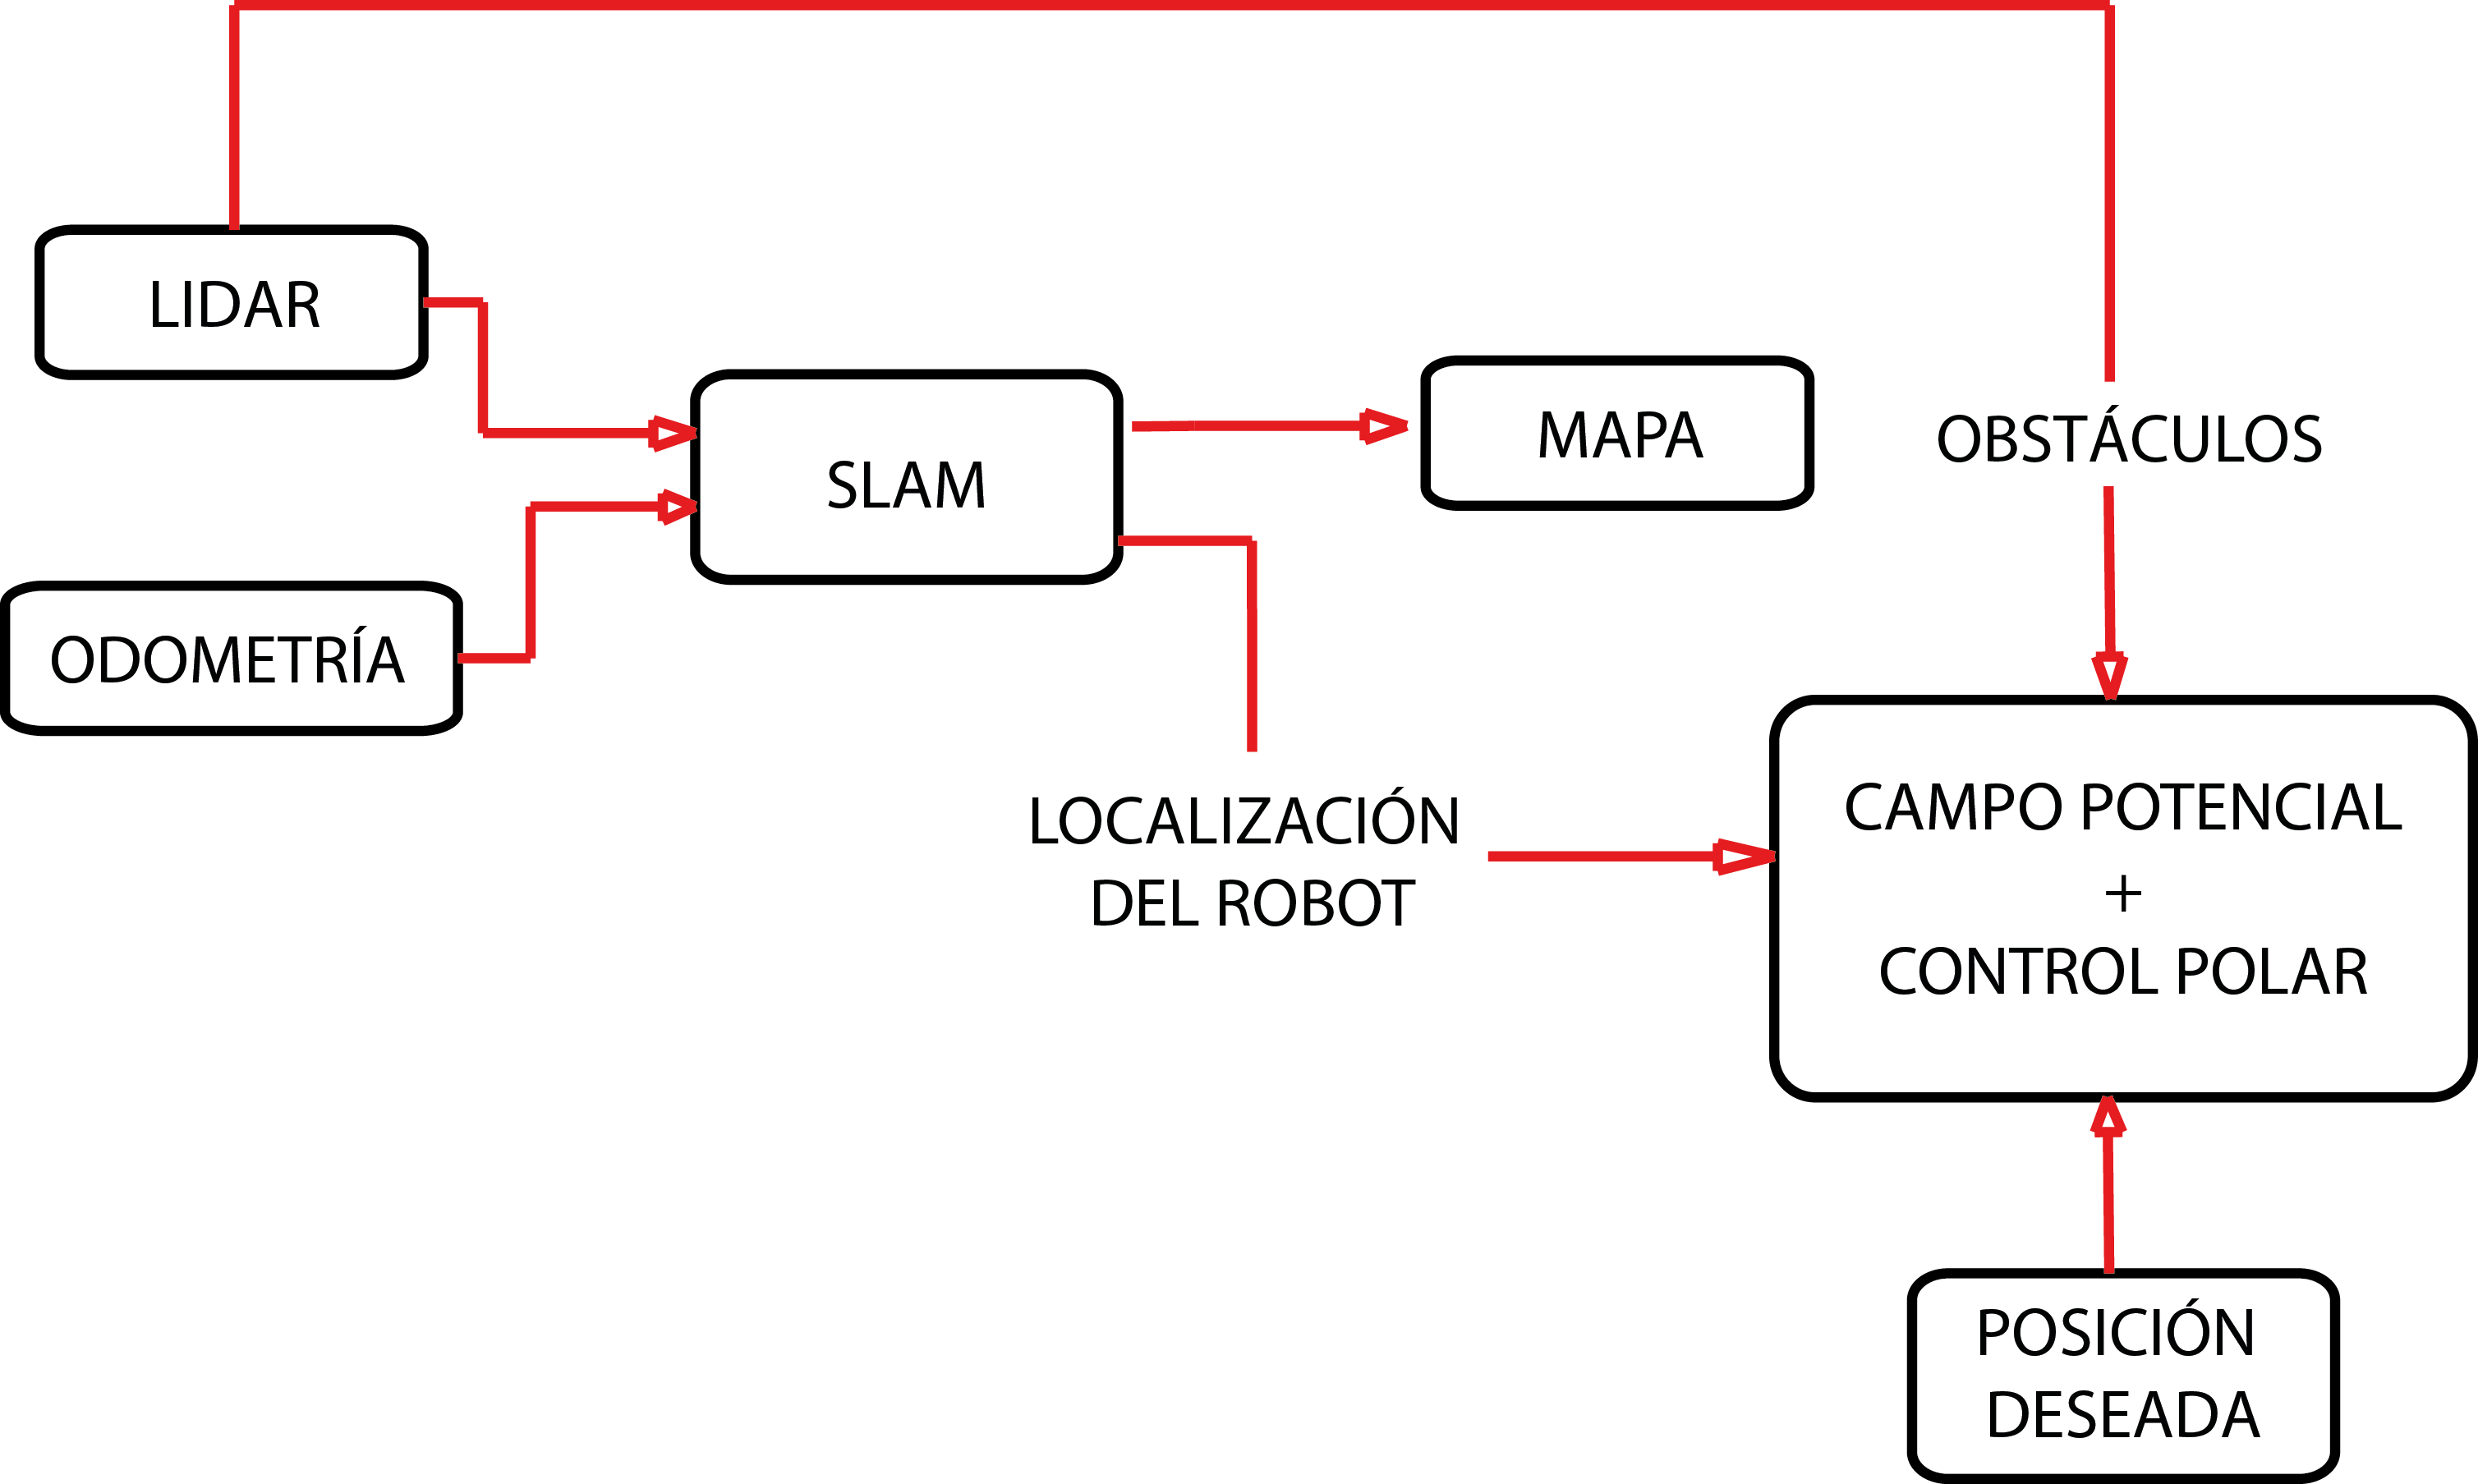
\includegraphics[width=0.9\textwidth]{images/estruct_auto.png}
	\captionsetup{font=footnotesize}
	\caption{Arquitectura de control del sistema para la autonomía de un robot móvil}
	\label{fig:ArqSist}
\end{figure}
 
Para que el robot se localicé dentro de un ambiente desconocido, se utiliza el bloque del SLAM. 
Este algoritmo tiene como entradas los datos del sensor lidar y de la odometría del robot 
($x_{medido},y_{medido},\theta_{medido}$). El SLAM con los datos mencionados utilza filtros de 
partículas y puede corregir la posición del robot dentro del ambiente desconocido. El 
bloque de SLAM tiene como salidas el mapa en dos dimensiones del lugar y la localización del robot 
corregido ($x_{corregido},y_{corregido},\theta_{corregido}$). El mapa en dos dimensiones permite
visualizar el entorno, en tiempo real, que se esta explorando.

El bloque del campo potencial más control polar es la representación del algoritmo utilizado
para la generación de trayectoria. Este algoritmo tiene como entradas los datos del sensor 
lidar, la localización corregida del robot y la posición deseada. El algoritmo trabaja de forma 
iterativa, tomando en consideración los obstáculos y la posición deseada. Para la exlporación del 
robot dentro del ambiente desconocido, se toma posiciones deseadas de forma aleatoria que son
entradas del algoritmo y a través de los campos potenciales el robot puede llegar hacia la posición 
deseada. En el caso de que el robot mientras se va moviendo el sensor lidar detecte un obstáculo, 
este enviará las posiciones del obstáculo y el algoritmo evitará que el robot se choque y a su vez
pide una nueva posición deseada para que pueda crear una nueva trayectoria y seguir explorando el 
ambiente. El controlador polar es utilizado para que el robot pueda moverse de forma suave en las 
curvas que se forman al generar su propia trayectoria.

Finalmente, el algoritmo de la generación de trayectoria tiene como salida la velocidad lineal y 
velocidad angular que debe tener el robot para desplazarse dentro del ambiente que esta explorando. Todo 
el sistema de navegación autónoma para el robot móvil se hace de forma iterativa hasta que el robot 
termine de mapear todo el ambiente, una vez culminado el robot regresa hacia su posición inicial. El 
sistema de navegación se puede ver en la figura \ref{fig:ArqSist}.


\subsection{Arquitectura del Sistema de Mapeo en Tres Dimensiones}

\begin{figure}%[ht!]
	\centering \footnotesize
	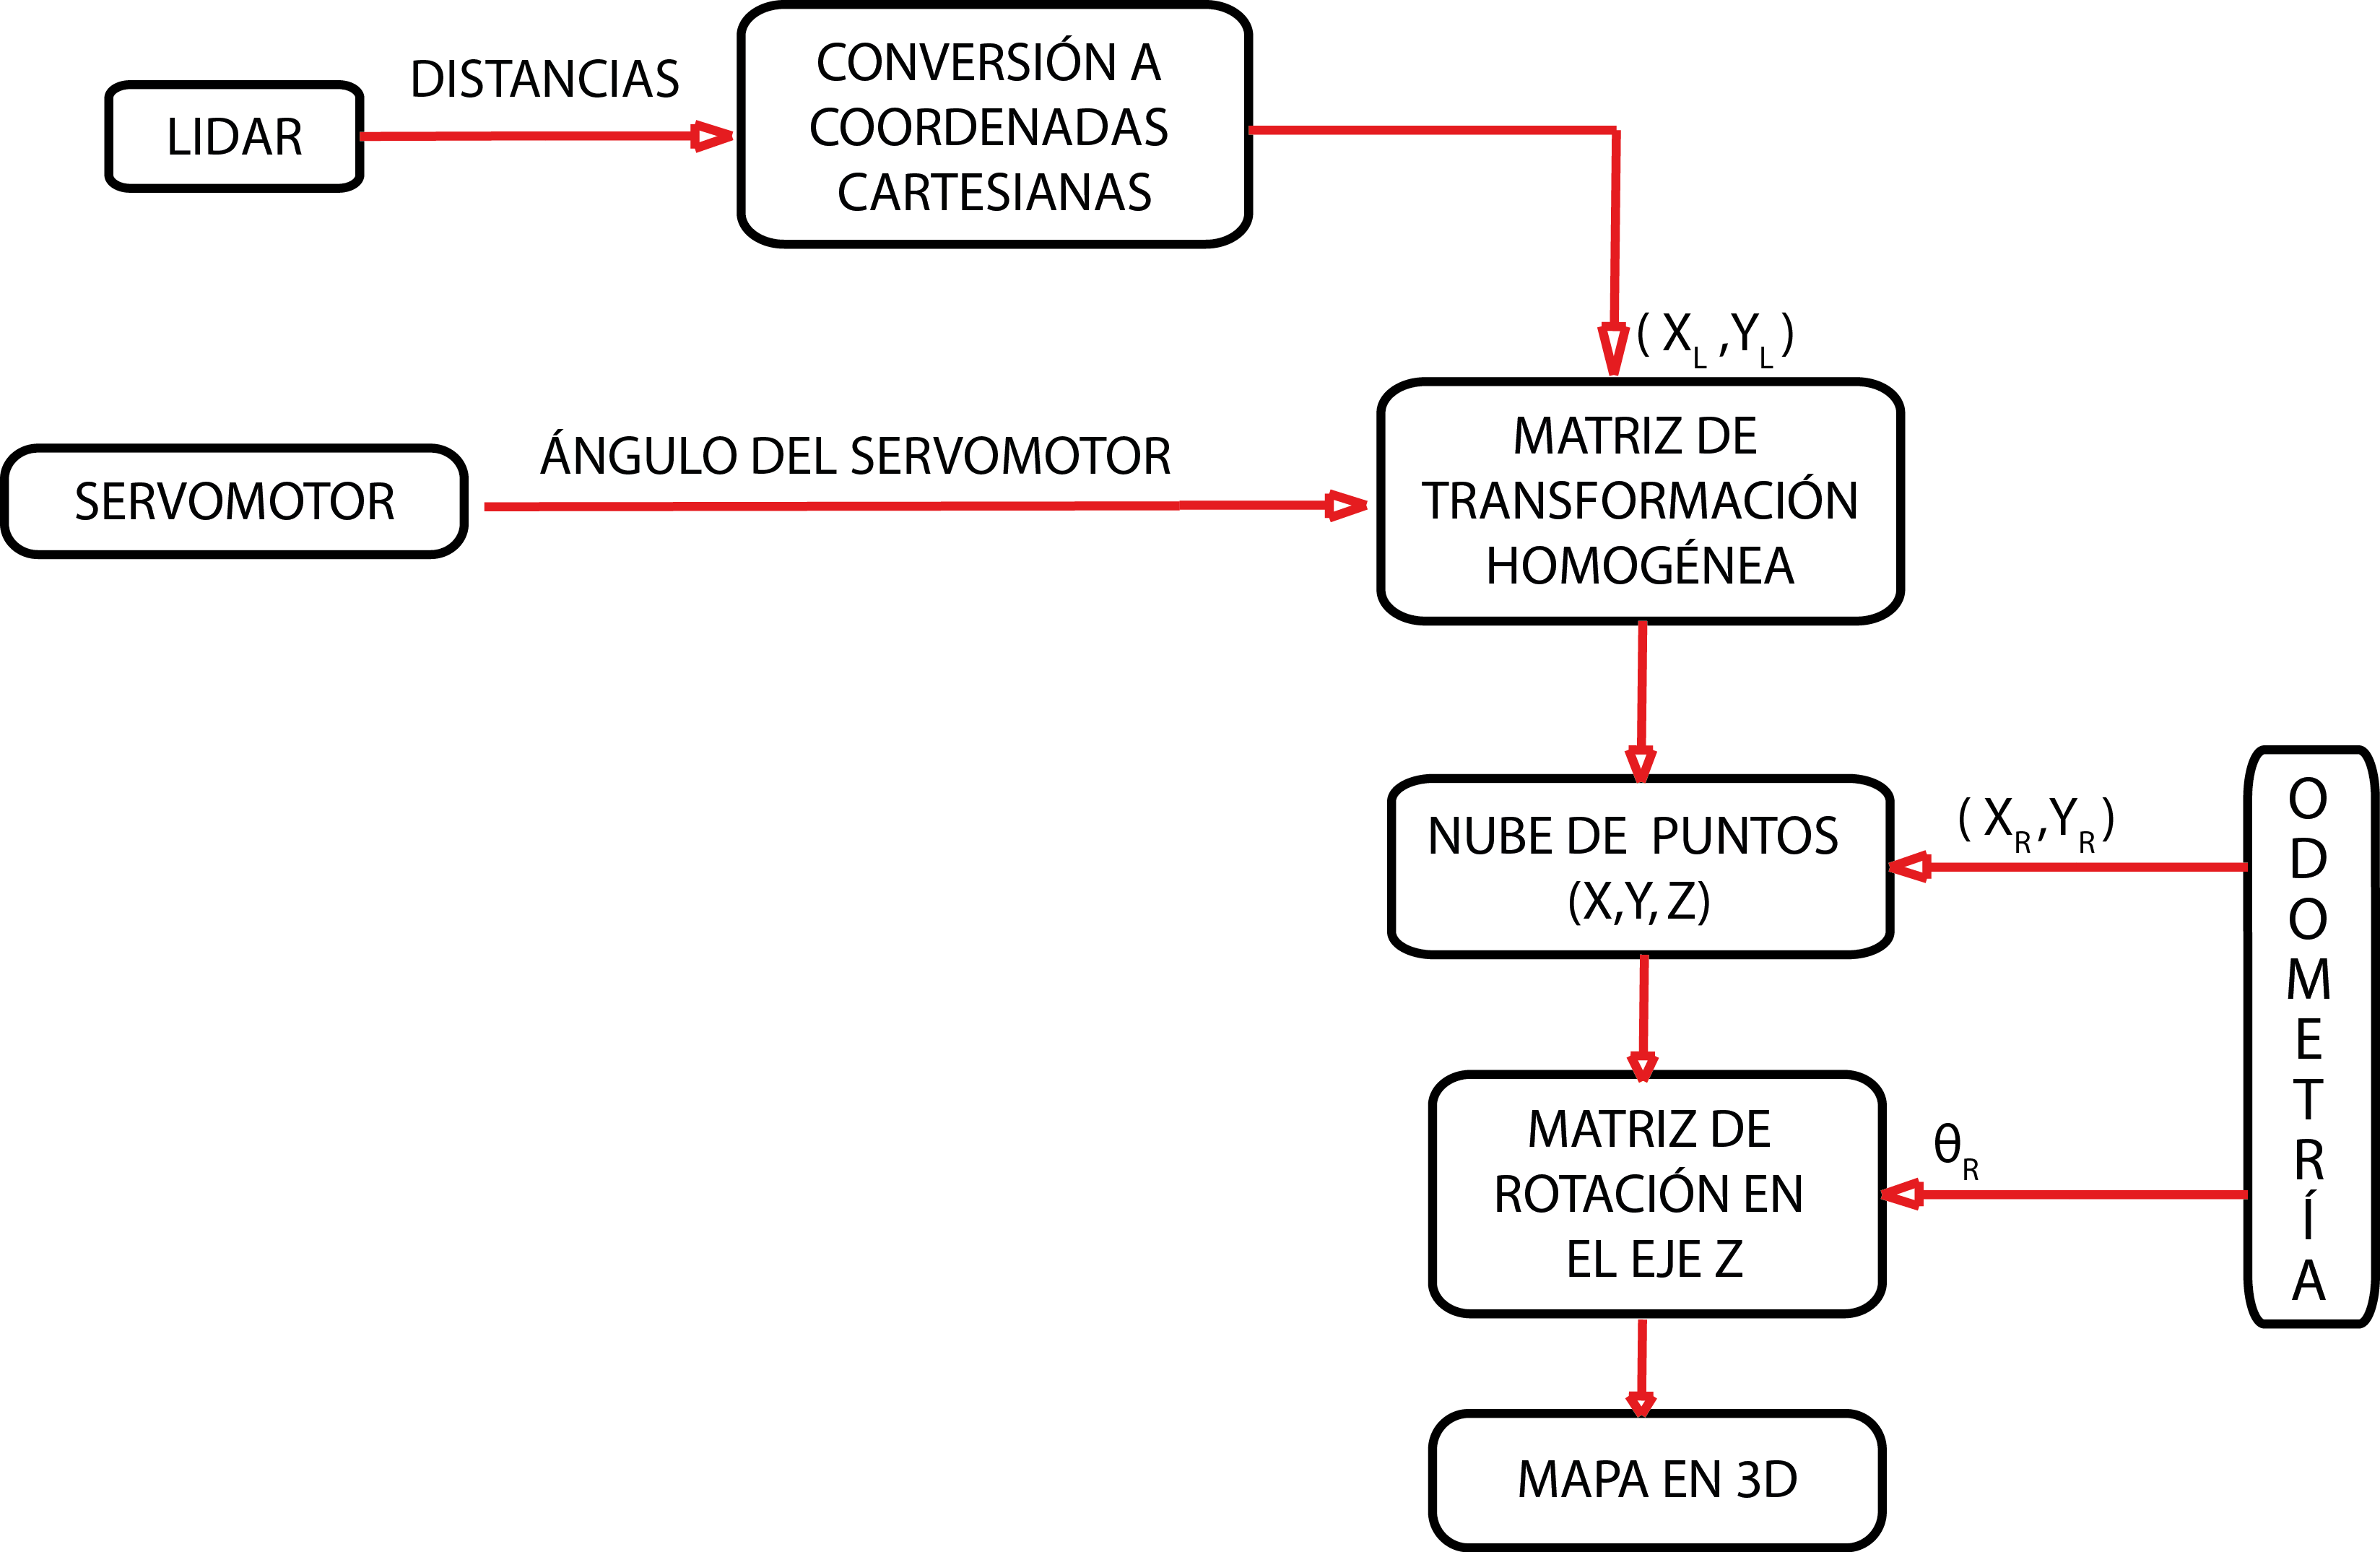
\includegraphics[width=0.9\textwidth]{images/estructura_3d.png}
	\captionsetup{font=footnotesize}
	\caption{Arquitectura del sistema de mapeo en 3D con un robot móvil}
	\label{fig:Sist3D}
\end{figure}

En esta parte del trabajo de tesis se muestra la estructura del sistema para realizar el
mapa en tres dimensiones. La estructura se muestra en la figura \ref{fig:Sist3D}. Este 
proceso comienza con las medidas que genera el sensor lidar, estas mediciones tienen
que ser convertidas en posiciones dentro de las coordenadas cartesianas en dos dimensiones
($X_{L}, Y_{L}$). La conversión a coordenadas polares permite conocer las posiciones de los 
obstáculos dentro de un ambiente y asimismo conocer las dimensiones del entorno que se esta 
explorando.

Para obtener la nube de puntos, se necesita los ángulos de rotación del servomotor. El 
servomotor hace rotar el sistema mecánico descrito y explicado en la sección 
\ref{sec:SistP3D}. El sistema mecánico implementado tiene un movimiento de rotación y otro 
de traslación. El sistema de referencia del sensor lidar se toma como el 
sistema de referencia del servomotor. Por tal motivo se utiliza una matriz de transformación 
homogénea, la cual esta compuesta por una matriz de rotación en el eje $Y_{S}$ del servomotor 
y una matriz de traslación con un desplazamiento en el eje $Z_{S}$ del servomotor. El
servomotor hace que el sensor lidar tenga un ángulo de abertura de 30\grad~ que permite
hacer mediciones en el eje $Z$. El resultado de la multiplicación de las posiciones 
($X_{L}, Y_{L}$) del sensor lidar con la matriz de transformación homogénea es
una nube de puntos ($X_{M}, Y_{M}, Z_{M}$) del mapa del entorno.

El robot explora el entorno y a su vez va realizando el mapa en tres dimensiones de las zonas
exploradas. El mapa debe tener correlación con la trayectoria que realiza el movimiento del 
robot, para esto se debe sumar los valores de la odometría del robot móvil. La odometría del 
robot es la estimación de la posición y orientación del robot mientras este se encuentra 
navegando dentro de un ambiente. La odometría esta compuesta por tres valores ($X_{R}, Y_{R}, 
\theta_{R}$). Para que el mapa pueda tener las posiciones con mayor precisión se suma los 
valores de ($X_{R}, Y_{R}$) del robot a la nube de puntos del mapa tridimensional. Otra
consideración en la construcción del mapa es la rotación del robot móvil al momento de 
realizar giros en su propio eje $Z_{R}$. Para este caso se utiliza el valor del ángulo 
de rotación ($\theta_{R}$) en una matriz de rotación del eje $Z$. Finalmente la nueva nube 
de puntos multiplicado con la matriz de rotación en el eje $Z_{R}$ del robot, genera el mapa 
en tres dimensiones de la zona explorada.
